%%%%%%%%%%%%%%%%%%%%%%%%%%%%%%%%%%%%%%%%%%%%%%%%%%%%%%%%%%%%%%%%%%%%%%%%%
%  Zawartość: Główny plik szablonu pracy dyplomowej (magisterskiej/inżynierskiej).
%  Opracował: Tomasz Kubik <tomasz.kubik@pwr.edu.pl>
%  Data: kwiecień 2016
%  Wersja: 0.2
%%%%%%%%%%%%%%%%%%%%%%%%%%%%%%%%%%%%%%%%%%%%%%%%%%%%%%%%%%%%%%%%%%%%%%%%%

\documentclass[a4paper,onecolumn,oneside,12pt,extrafontsizes]{memoir}
% W celu przygotowania wydruku do archiwum należy przesłonić komendę powyższą
% dwoma poniższymi komendami:
%\documentclass[a4paper,onecolumn,twoside,10pt]{memoir} 
%\renewcommand{\normalsize}{\fontsize{8pt}{10pt}\selectfont}

%\usepackage[cp1250]{inputenc} % jeśli kodowanie edytowanych plików to cp1250 
\usepackage[utf8]{inputenc} % jeśli kodowanie edytowanych plików to UTF8
\usepackage[T1]{fontenc}
%\DisemulatePackage{setspace}
\usepackage{setspace}
\usepackage{tabularx}
\usepackage{color,calc}
%\usepackage{soul} % pakiet z komendami do podkreślania tekstu

\usepackage{ebgaramond} % pakiet z czcionkami garamond, potrzebny tylko do strony tytułowej, musi wystąpić przed pakietem tgtermes

%% Aby uzyskać polskie literki w pdfie (a nie zlepki) korzystamy z pakietu czcionek tgterms. 
%% W pakiecie tym są zdefiniowane klony czcionek Times o kształtach: normalny, pogrubiony, italic, italic pogrubiony.
%% W pakiecie tym brakuje czcionki o kształcie: slanted (podobny do italic). 
%% Jeśli w dokumencie gdzieś zostanie zastosowana czcionka slanted (np. po użyciu komendy \textsl{}), to
%% latex dokona podstawienia na czcionkę standardową i zgłosi to w ostrzeżeniu (warningu).
%% Ponadto tgtermes to czcionka do tekstu. Wszelkie matematyczne wzory będą sformatowane domyślną czcionką do wzorów.
%% Jeśli wzory mają być sformatowane z wykorzystaniem innych czcionek, trzeba to jawnie zadeklarować.

%% Po zainstalowaniu pakietu tgtermes może będzie trzeba zauktualizować informacje 
%% o dostępnych fontach oraz mapy. Można to zrobić z konsoli (jako administrator)
%% initexmf --admin --update-fndb
%% initexmf --admin --mkmaps

\renewcommand*\ttdefault{txtt}

% We wcześniejszej wersji szablonu korzystano z innych czcionek. Dla celów historycznych pozostawiono je w komentarzu
%\usepackage{mathptmx} % pakiet będący następcą pakietów times and mathptm, niestety polskie literki są zlepkami
%\usepackage{newtxtext,newtxmath} % pakiety dostarczające Times dla tekstów i wzorów matematycznych,  
%                                  rozwiązuje problemy występujące w mathptmx, ale wymaga zainstalowania
%                                  dodatkowych pakietów oraz uruchomienia updmap (konsola administratora)
%                                  niestety polskie literki są zlepkami
%\usepackage{newtxmath,tgtermes} % można też połączyć czcionki do tekstu i czcionki do wzorów

\usepackage{listings} % pakiet do prezentacji kodu. 
%Wcześniej był problem z polskimi znakami w otoczeniu lstlisting, stąd pozostawiono w komentarzu zastosowane wtedy rozwiązanie: 
\lstset{literate=%-
{ą}{{\k{a}}}1 {ć}{{\'c}}1 {ę}{{\k{e}}}1 {ł}{{\l{}}}1 {ń}{{\'n}}1 {ó}{{\'o}}1 {ś}{{\'s}}1 {ż}{{\.z}}1 {ź}{{\'z}}1 {Ą}{{\k{A}}}1 {Ć}{{\'C}}1 {Ę}{{\k{E}}}1 {Ł}{{\L{}}}1 {Ń}{{\'N}}1 {Ó}{{\'O}}1 {Ś}{{\'S}}1 {Ż}{{\.Z}}1 {Ź}{{\'Z}}1 }%{\ \ }{{\ }}1}

% Choć możliwe jest zastosowanie różnych pakietów formatujących tabele, zaleca się tego nie robić.
%\usepackage{longtable}
%\usepackage{ltxtable}
%\usepackage{tabulary}

%%%%%%%%%%%%%%%%%%%%%%%%%%%%%%%%%%%%%%%%%%%%%%%%%%%
%% Ustawienia odpowiedzialne za sposób łamania dokumentu
%% i ułożenie elementów pływających
%%%%%%%%%%%%%%%%%%%%%%%%%%%%%%%%%%%%%%%%%%%%%%%%%%%
%\hyphenpenalty=10000		% nie dziel wyrazów zbyt często
\clubpenalty=10000      %kara za sierotki
\widowpenalty=10000  % nie pozostawiaj wdów
\brokenpenalty=10000		% nie dziel wyrazów między stronami
\exhyphenpenalty=999999		% nie dziel słów z myślnikiem
\righthyphenmin=3			% dziel minimum 3 litery

%\tolerance=4500
%\pretolerance=250
%\hfuzz=1.5pt
%\hbadness=1450

\renewcommand{\topfraction}{0.95}
\renewcommand{\bottomfraction}{0.95}
\renewcommand{\textfraction}{0.05}
\renewcommand{\floatpagefraction}{0.35}

%%%%%%%%%%%%%%%%%%%%%%%%%%%%%%%%%%%%%%%%%%%%%%%%%%%
%%  Ustawienia rozmiarów: tekstu, nagłówka i stopki, marginesów
%%  dla dokumentów klasy memoir 
%%%%%%%%%%%%%%%%%%%%%%%%%%%%%%%%%%%%%%%%%%%%%%%%%%%
\setlength{\headsep}{10pt} 
\setlength{\headheight}{13.6pt} % wartość baselineskip dla czcionki 11pt tj. \small wynosi 13.6pt
\setlength{\footskip}{\headsep+\headheight}
\setlength{\uppermargin}{\headheight+\headsep+1cm}
\setlength{\textheight}{\paperheight-\uppermargin-\footskip-1.5cm}
\setlength{\textwidth}{\paperwidth-5cm}
\setlength{\spinemargin}{2.5cm}
\setlength{\foremargin}{2.5cm}
\setlength{\marginparsep}{2mm}
\setlength{\marginparwidth}{2.3mm}
%\settrimmedsize{297mm}{210mm}{*}
%\settrims{0mm}{0mm}	
\checkandfixthelayout[fixed] % konieczne, aby się dobrze wszystko poustawiało
%%%%%%%%%%%%%%%%%%%%%%%%%%%%%%%%%%%%%%%%%%%%%%%%
%%  Ustawienia odległości linii, wcięć, odstępów
%%%%%%%%%%%%%%%%%%%%%%%%%%%%%%%%%%%%%%%%%%%%%%%%
\linespread{1}
%\linespread{1.241}
\setlength{\parindent}{14.5pt}
%\setbeforesecskip{10pt plus 0.5ex}%{-3.5ex \@plus -1ex \@minus -.2ex}
%\setaftersecskip{10pt plus 0.5ex}%\onelineskip}
%\setbeforesubsecskip{8pt plus 0.5ex}%{-3.5ex \@plus -1ex \@minus -.2ex}
%\setaftersubsecskip{8pt plus 0.5ex}%\onelineskip}
%\setlength\floatsep{6pt plus 2pt minus 2pt} 
%\setlength\intextsep{12pt plus 2pt minus 2pt} 
%\setlength\textfloatsep{12pt plus 2pt minus 2pt} 

%%%%%%%%%%%%%%%%%%%%%%%%%%%%%%%%%%%%%%%%%%%%%%%%%%%
%%  Pakiety i komendy zastosowane tylko do zamieszczenia informacji o użytych komendach i fontach
%%  Normalnie nie są potrzebne, można je zamarkować podczas redakcji pracy
%%%%%%%%%%%%%%%%%%%%%%%%%%%%%%%%%%%%%%%%%%%%%%%%%%%
\usepackage{memlays}     % extra layout diagrams, zastosowane w szblonie do 'debuggowania', używa pakietu layouts
%\usepackage{layouts}
\usepackage{printlen} % pakiet do wyświetlania wartości zdefiniowanych długości, stosowany do 'debuggowania'
\uselengthunit{pt}
\makeatletter
\newcommand{\showFontSize}{\f@size pt} % makro wypisujące wielkość bieżącej czcionki
\makeatother
% do pokazania ramek można byłoby użyć:
%\usepackage{showframe} 


%%%%%%%%%%%%%%%%%%%%%%%%%%%%%%%%%%%%%%%%%%%%%%%%%%%
%%  Formatowanie list wyliczeniowych, wypunktowań i własnych otoczeń
%%%%%%%%%%%%%%%%%%%%%%%%%%%%%%%%%%%%%%%%%%%%%%%%%%%

% Domyślnie wypunktowania mają zadeklatorowane znaki, które nie występują w tgtermes
% Aby latex nie podstawiał w ich miejsca znaków z czcionki standardowej można zrobić podstawienie:
%    \DeclareTextCommandDefault{\textbullet}{\ensuremath{\bullet}}
%    \DeclareTextCommandDefault{\textasteriskcentered}{\ensuremath{\ast}}
%    \DeclareTextCommandDefault{\textperiodcentered}{\ensuremath{\cdot}}
% Jednak jeszcze lepszym pomysłem jest zdefiniowanie otoczeń z wykorzystaniem enumitem
\usepackage{enumitem} % pakiet pozwalający zarządzać formatowaniem list wyliczeniowych
\setlist{noitemsep,topsep=4pt,parsep=0pt,partopsep=4pt,leftmargin=*} % zadeklarowane parametry pozwalają uzyskać 'zwartą' postać wypunktowania bądź wyliczenia
\setenumerate{labelindent=0pt,itemindent=0pt,leftmargin=!,label=\arabic*.} % można zmienić \arabic na \alph, jeśli wyliczenia mają być z literkami
\setlistdepth{4} % definiujemy głębokość zagnieżdżenia list wyliczeniowych do 4 poziomów
\setlist[itemize,1]{label=$\bullet$}  % definiujemy, jaki symbol ma być użyty w wyliczeniu na danym poziomie
\setlist[itemize,2]{label=\normalfont\bfseries\textendash}
\setlist[itemize,3]{label=$\ast$}
\setlist[itemize,4]{label=$\cdot$}
\renewlist{itemize}{itemize}{4}

%%%http://tex.stackexchange.com/questions/29322/how-to-make-enumerate-items-align-at-left-margin
%\renewenvironment{enumerate}
%{
%\begin{list}{\arabic{enumi}.}
%{
%\usecounter{enumi}
%%\setlength{\itemindent}{0pt}
%%\setlength{\leftmargin}{1.8em}%{2zw} % 
%%\setlength{\rightmargin}{0zw} %
%%\setlength{\labelsep}{1zw} %
%%\setlength{\labelwidth}{3zw} % 
%\setlength{\topsep}{6pt}%
%\setlength{\partopsep}{0pt}%
%\setlength{\parskip}{0pt}%
%\setlength{\parsep}{0em} % 
%\setlength{\itemsep}{0em} % 
%%\setlength{\listparindent}{1zw} % 
%}
%}{
%\end{list}
%}

\makeatletter
\renewenvironment{quote}{
	\begin{list}{}
	{
	\setlength{\leftmargin}{1em}
	\setlength{\topsep}{0pt}%
	\setlength{\partopsep}{0pt}%
	\setlength{\parskip}{0pt}%
	\setlength{\parsep}{0pt}%
	\setlength{\itemsep}{0pt}
	}
	}{
	\end{list}}
\makeatother

%%%%%%%%%%%%%%%%%%%%%%%%%%%%%%%%%%%%%%%%%
%%  Pakiet do generowania indeksu (ważne, aby wstawić przed hyperref)
%%%%%%%%%%%%%%%%%%%%%%%%%%%%%%%%%%%%%%%%%
\DisemulatePackage{imakeidx}
\usepackage[makeindex,noautomatic]{imakeidx} % tutaj mówimy, żeby indeks nie generował się automatycznie, 

%\usepackage[noautomatic]{imakeidx} 
\makeindex

\makeatletter
%%%\renewenvironment{theindex}
							 %%%{\vskip 10pt\@makeschapterhead{\indexname}\vskip -3pt%
								%%%\@mkboth{\MakeUppercase\indexname}%
												%%%{\MakeUppercase\indexname}%
								%%%\vspace{-3.2mm}\parindent\z@%
								%%%\renewcommand\subitem{\par\hangindent 16\p@ \hspace*{0\p@}}%%
								%%%\phantomsection%
								%%%\begin{multicols}{2}
								%%%%\thispagestyle{plain}
								%%%\parindent\z@                
								%%%%\parskip\z@ \@plus .3\p@\relax
								%%%\let\item\@idxitem}
							 %%%{\end{multicols}\clearpage}
%%%
\makeatother


\usepackage{ifpdf}
%\newif\ifpdf \ifx\pdfoutput\undefined
%\pdffalse % we are not running PDFLaTeX
%\else
%\pdfoutput=1 % we are running PDFLaTeX
%\pdftrue \fi
\ifpdf
 \usepackage[pdftex,bookmarks,breaklinks,unicode]{hyperref}
 \usepackage[pdftex]{graphicx}
 \DeclareGraphicsExtensions{.pdf,.jpg,.mps,.png}
\pdfcompresslevel=9
\pdfoutput=1
\makeatletter
\AtBeginDocument{
  \hypersetup{
	pdfinfo={
    Title = {\@title},
    Author = {\@author},
    Subject={},
    Keywords={słowa kluczowe},
  }}
}
\makeatother
\else
\usepackage{graphicx}
\DeclareGraphicsExtensions{.eps,.ps,.jpg,.mps,.png}
\fi
\sloppy


%\graphicspath{{rys01/}{rys02/}}


%%%%%%%%%%%%%%%%%%%%%%%%%%%%%%%%%%%%%%%%%
% Metadane dla pdfa


%\ifpdf
%\pdfinfo{
   %/Author (Nicola Talbot)
   %/Title  (Creating a PDF document using PDFLaTeX)
   %/CreationDate (D:20040502195600)
   %/ModDate (D:\pdfdate)
   %/Subject (PDFLaTeX)
   %/Keywords (PDF;LaTeX)
%}
%\fi

% Deklaracja głębokościu numeracji
\setcounter{secnumdepth}{2}
\setcounter{tocdepth}{2}
\setsecnumdepth{subsection} % activating subsubsec numbering in doc


% Kropki po numerach sekcji
\makeatletter
\def\@seccntformat#1{\csname the#1\endcsname.\quad}
\def\numberline#1{\hb@xt@\@tempdima{#1\if&#1&\else.\fi\hfil}}
\makeatother

\renewcommand{\chapternumberline}[1]{#1.\quad}
\renewcommand{\cftchapterdotsep}{\cftdotsep}

%\definecolor{niceblue}{rgb}{.168,.234,.671}

% Czcionka do podpisów tabel i rysunków
\captionnamefont{\small}
\captiontitlefont{\small}
% makro pozwalające zmienić sposób wypisywania rozdziału
%\def\printchaptertitle##1{\fonttitle \space \thechapter.\space ##1} 

%\usepackage{ltcaption}
% The ltcaption package supports \CaptionLabelFont & \CaptionTextFont introduced by the NTG document classes
%\renewcommand\CaptionLabelFont{\small}
%\renewcommand\CaptionTextFont{\small}
%%%%%%%%%%%%%%%%%%%%%%%%%%%%%%%%%%%%%%%%%%%%%%%%%%%%%%%%%%%%%%%%%%                  
%% Definicje stopek i nagłówków
%%%%%%%%%%%%%%%%%%%%%%%%%%%%%%%%%%%%%%%%%%%%%%%%%%%%%%%%%%%%%%%%%%                  
%%%%%%%%%%%%%%%%%%%%%%%%%%%%%%%%%%%%%%%
%% Definicja strony tytułowej 
%%%%%%%%%%%%%%%%%%%%%%%%%%%%%%%%%%%%%%%
\makeatletter
%Uczelnia
\newcommand\uczelnia[1]{\renewcommand\@uczelnia{#1}}
\newcommand\@uczelnia{}
%Wydział
\newcommand\wydzial[1]{\renewcommand\@wydzial{#1}}
\newcommand\@wydzial{}
%Kierunek
\newcommand\kierunek[1]{\renewcommand\@kierunek{#1}}
\newcommand\@kierunek{}
%Specjalność
\newcommand\specjalnosc[1]{\renewcommand\@specjalnosc{#1}}
\newcommand\@specjalnosc{}
%Tytuł po angielsku
\newcommand\titleEN[1]{\renewcommand\@titleEN{#1}}
\newcommand\@titleEN{}
%Tytuł krótki
\newcommand\titleShort[1]{\renewcommand\@titleShort{#1}}
\newcommand\@titleShort{}
%Promotor
\newcommand\promotor[1]{\renewcommand\@promotor{#1}}
\newcommand\@promotor{}

%\usepackage[absolute]{textpos} % zamarkowano, bo ostatecznie wykorzystano otoczenie picture

\def\maketitle{%
  \pagestyle{empty}%
%%\garamond 
	\fontfamily{\ebgaramond@family}\selectfont % na stronie tytułowej czcionka garamond
%%%%%%%%%%%%%%%%%%%%%%%%%%%%%%%%%%%%%	
%% Poniżej, w otoczniu picture, wstawiono tytuł i autora. 
%% Tytuł (z autorem) musi znaleźć się w obszarze 
%% odpowiadającym okienku 110mmx75mm, którego lewy górny róg 
%% jest w położeniu 77mm od lewej i 111mm od górnej  krawędzi strony 
%% (tak wynika z wycięcia na okładce). 
%% Poniższy kod musi być użyty dokładnie w miejscu gdzie jest.
%% Jeśli tytuł nie mieści się w okienku, to należy tak pozmieniać 
%% parametry użytych komend, aby ten przydługi tytuł jednak 
%% upakować go do okienka.
%%
%% Sama okładka (kolorowa strona z wycięciem, do pobrania z dydaktyki) 
%% powinna być przycięta o 3mm od każdej z krawędzi.
%% Te 3mm pewnie zostawiono na ewentualne spady czy też specjalną oprawę.
%%%%%%%%%%%%%%%%%%%%%%%%%%%%%%%%%%%%%	
\newlength{\tmpfboxrule}
\setlength{\tmpfboxrule}{\fboxrule}
\setlength{\fboxsep}{2mm}
\setlength{\fboxrule}{0mm} 
%\setlength{\fboxrule}{0.1mm} %% jeśli chcemy zobaczyć ramkę
\setlength{\unitlength}{1mm}
\begin{picture}(0,0)
\put(26,-124){\fbox{
\parbox[c][71mm][c]{104mm}{\centering%\lineskip=34pt 
\fontsize{16pt}{18pt}\selectfont \@title\\[5mm]
\fontsize{16pt}{18pt}\selectfont AUTHOR:\\[2mm]
\fontsize{14pt}{16pt}\selectfont \@author}
}
}
\end{picture}
\setlength{\fboxrule}{\tmpfboxrule} 
%%%%%%%%%%%%%%%%%%%%%%%%%%%%%%%%%%%%%
%% Reszta strony z nazwą uczelni, wydziału, kierunkiem, specjalnością
%% promotorem, oceną pracy, miastem i rokiem
	{\centering%\vspace{-1cm}
		{\fontsize{22pt}{24pt}\selectfont \@uczelnia}\\[0.4cm]
		{\fontsize{22pt}{24pt}\selectfont \@wydzial}\\[0.5cm]
		  \hrule %\vspace*{0.7cm}
	}
{\flushleft\fontsize{14pt}{16pt}\selectfont%
\begin{tabular}{ll}
FIELD OF STUDY: & \@kierunek\\
SPECIALITY: & \@specjalnosc\\
\end{tabular}\\[1.3cm]
}
{\centering
{\fontsize{32pt}{36pt}\selectfont ENGINEERING}\\[0.5cm]
{\fontsize{32pt}{36pt}\selectfont THESIS}\\[2.5cm]
}
\vfill
\begin{tabularx}{\linewidth}{p{6cm}l}
		&{\fontsize{16pt}{18pt}\selectfont THESIS SUPERVISOR:}\\[2mm] %UWAGA: tutaj jest miejsce na nazwisko promotora pracy
		&{\fontsize{14pt}{16pt}\selectfont \@promotor}\\[10mm]
	\end{tabularx}
\vspace{2cm}
\hrule\vspace*{0.3cm}
{\centering
{\fontsize{16pt}{18pt}\selectfont \@date}\\[0cm]
}
%\ungaramond
\normalfont
 \cleardoublepage
}
\makeatother
%%%%%%%%%%%%%%%%%%%%%%%%%%%%%%%%%%%%%%%%%

%\AtBeginDocument{\addtocontents{toc}{\protect\thispagestyle{empty}}}




%%%%%%%%%%%%%%%%%%%%%%%%%%%%%%%%%%%%%%%%%
%%  Metadane dokumentu 
%%%%%%%%%%%%%%%%%%%%%%%%%%%%%%%%%%%%%%%%%
\title{Application interface to control the SimBaD cancer cell proliferation simulator}
\titleShort{SimBaD simulator interface ...}
\author{Jakub Sokołowski}
\uczelnia{WROCŁAW UNIVERSITY OF TECHNOLOGY}
\wydzial{FACULTY OF ELECTRONICS}
\kierunek{COMPUTER ENGINEERING}
\specjalnosc{INTERNET ENGINEERING}
\promotor{Dr inż, Marek Bawiec}
\date{WROCŁAW, 2019}

% Ustawienie odstępu od góry w nienumerowanych rozdziałach oraz wykazach:
% Spis treści, Spis tabel, Spis rysunków, Indeks rzeczowy

%\newlength{\linespace}
%\setlength{\linespace}{-\beforechapskip-\topskip+\headheight+\topsep}
%\makechapterstyle{noNumbered}{%
%\renewcommand\chapterheadstart{\vspace*{\linespace}}
%}

%% powyższa komenda załatwia to, co robią komendy poniższe dla spisów
%\renewcommand*{\tocheadstart}{\vspace*{\linespace}}
%\renewcommand*{\lotheadstart}{\vspace*{\linespace}}
%\renewcommand*{\lofheadstart}{\vspace*{\linespace}}

%%%%%%%%%%%%%%%%%%%%%%%%%%%%%%%%%%%%%%%%%
%                  Początek dokumentu 
%%%%%%%%%%%%%%%%%%%%%%%%%%%%%%%%%%%%%%%%%
%\includeonly{skroty,rozdzial01} % jeśli chcemy kompilować tylko fragmenty, to można tu je wpisać

\begin{document}
% Tutaj można przełączyć odstęp między liniami
%\SingleSpacing
%\OnehalfSpacing
%\DoubleSpacing

%\settypeoutlayoutunit{cm} % do debugowania
%\typeoutstandardlayout    % wypisuje na stdout informacje o ustawieniach
\maketitle
% \newpage


% \chapterstyle{noNumbered}
% \pagestyle{outer}
% \mbox{}\pdfbookmark[0]{Spis treści}{spisTresci.1}
 \tableofcontents* 

 \newpage
 \mbox{}\pdfbookmark[0]{Spis rysunków}{spisRysunkow.1}
% %\addcontentsline{toc}{chapter}{Spis rysunków}
\listoffigures*
% \begin{flushleft}

% \end{flushleft}

% \newpage
% \mbox{}\pdfbookmark[0]{Spis tabel}{spisTabel.1}
% %\addcontentsline{toc}{chapter}{Spis tabel}
% \listoftables*

% \chapter*{List of Terms}\mbox{}\pdfbookmark[0]{Acronyms}{Acronyms.1}
\label{sec:skroty}
\noindent
\begin{description}
  \item [SimBad] (\emph{Simulation Birth and Death})
  \item [CLI] (\emph{Command Line Interface})
  \item [VM] (\emph{Virtual Machine})
  \item [OS] (\emph{Operating System })
\end{description}


\chapter{Introduction}
\section{SimBad project}
The SimBad project (Simulation Birth and Death) is a systems of several applications used in cancer cell proliferation simulations. Cancer cell proliferation simply is a  process of cell growth and division. Abnormal cell proliferation, that is, when  cells that divide only finite amount of time before halting their growth or simply dying start untamed proliferation it may cause cancer development.

The SimBad project is a set of applications developed to simulate such processes. It consists of three primary component - simulation program that runs simulation and generates output stream data - (SimBaD-CLI), simulation output analyzer (SimBaD- analyzer) and plot generator (SimBad-Reports). Components exchange information in pipeline-like way, each component recives some input file (or files) and based on those files it generates some output.

The process of simulation is as follows: it starts with a configuration file in which several dozen objects and parameters that determine the process of simulation. Around ~100 parameter that need to be set and adjusted in order to run simulation. Valid configuration is passed as input to SimBad-CLI which starts the simulation process. The output of CLI step is a .csv file which i turn is input of analyzer step. Form the .csv file, the analyzer step generates multiple .csv and .parquet files, which in turn are necessary to generate plots
in report step.

\begin{figure}[ht]
	\centering
		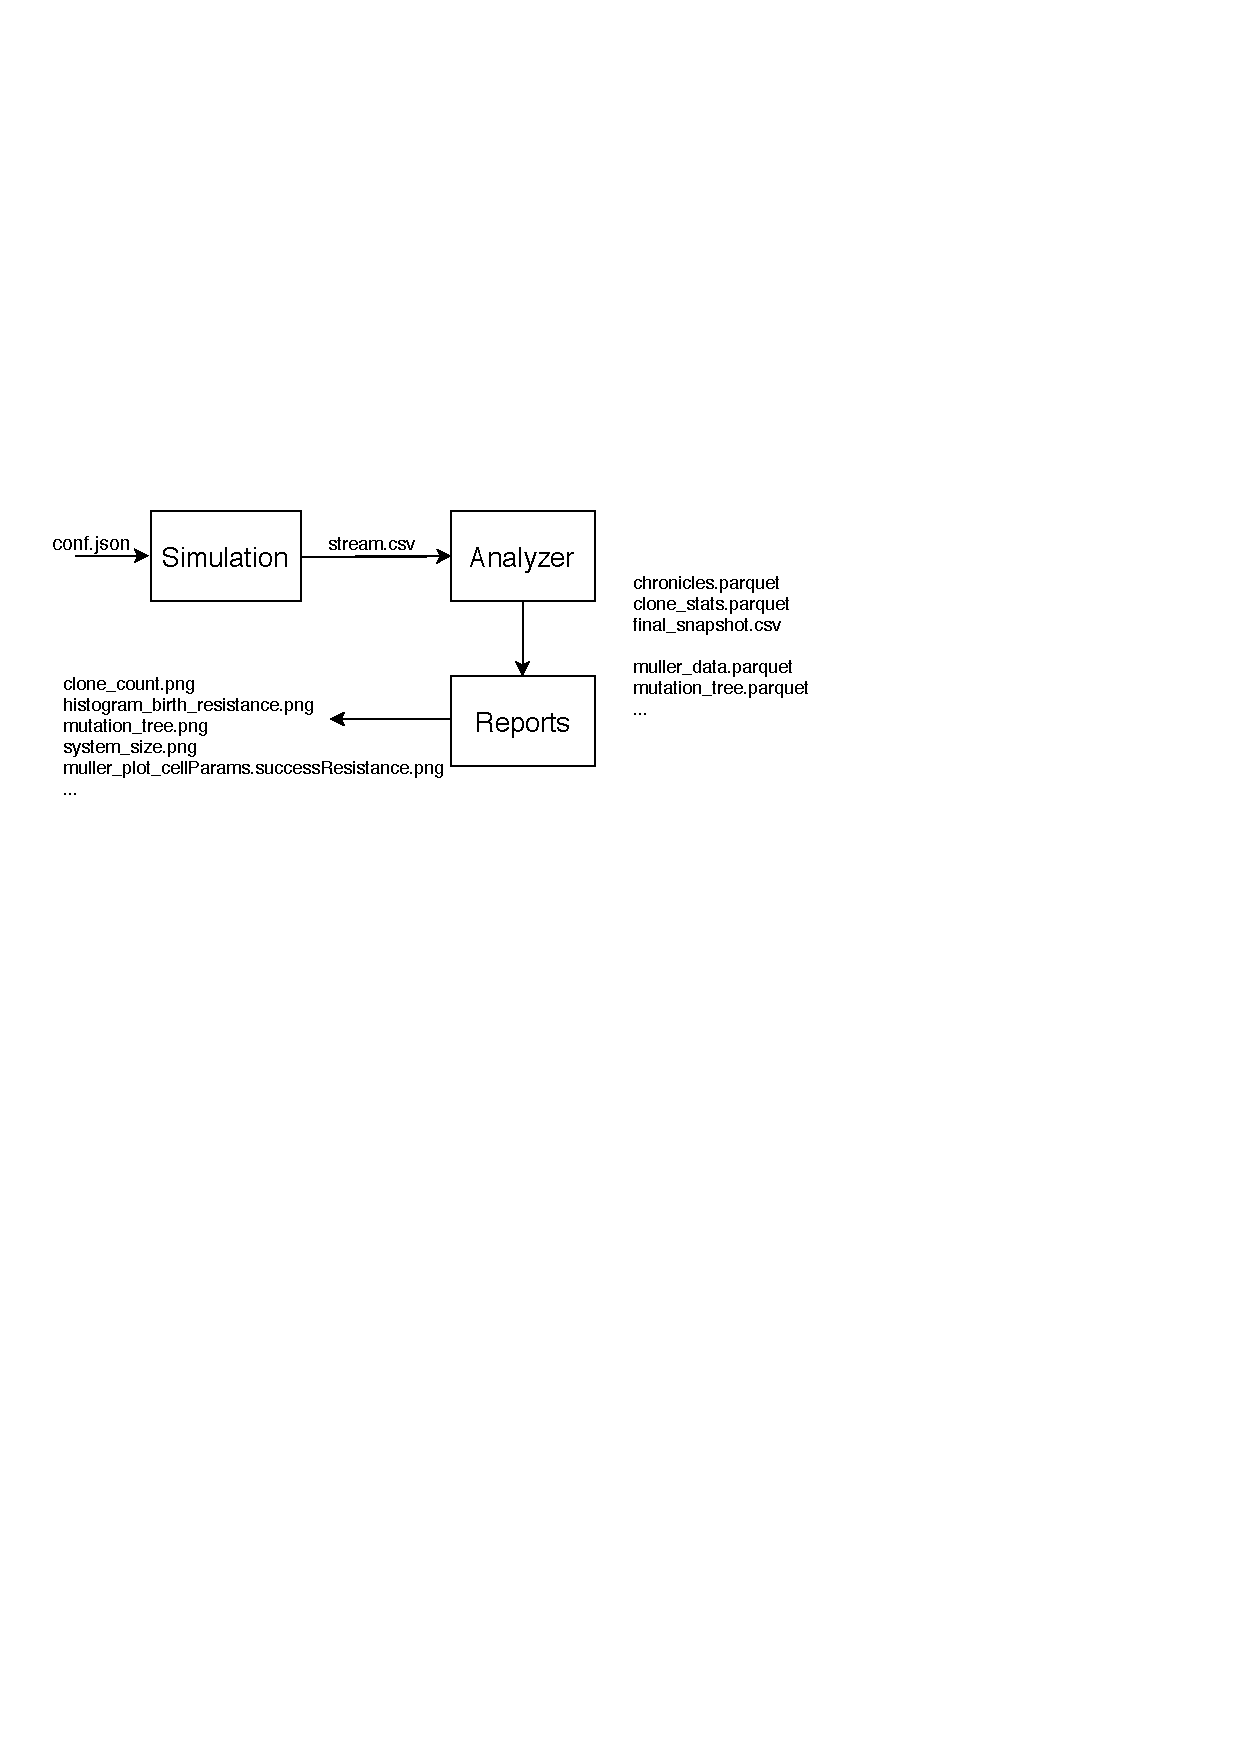
\includegraphics[width=0.9\linewidth]{diagrams/simbad-data-flow.pdf}
	\caption{Data flow between system components}
	\label{fig:data-flow}
\end{figure}

Each step has many dependencies on external libraries that need to be installed on host system and many configuration options that need to be set in order to execute the step. Due to high complexity of system, substantial amount of technical knowledge is needed to run the simulation process, and non-technical user are effectively unable to use this system, without help and guidance of its authors. Moreover, even if the user has required knowledge and skills to install and configure the system, system dependency on third-party code libraries that are not compatible with user machine may prevent the usage of the system.

To enable to users to use this system, an ease to use interface that will allow to control and monitor SimBad simulation process, and ability to install the system in host agnostic way are needed. The purpose of this thesis is to propose and implement such interface. 
Apart of ease of use, several other assumptions were made:
\begin{itemize}
    \item additional system components will be build on top of existing components without modifying them
    \item minimizing the resource footprint on host system
    \item host-agnostic installation
    \item decoupling of components
    \item zero-configuration needed for normal user and extensive configuration available to power user
\end{itemize}
In this thesis I will address each of those assumptions
\chapter{Existing system}
The main source of complexity of existing system are each component dependencies and managing them. Numerous dependencies must be installed on host operating system. The SimBaD project is still under development and new features are being added, and that causes a need for already installed components to be updated. Moreover, updates to host operating system may also evoke a need to update. To facilitate installation and updates of system, some kind of method of managing the project with its dependencies and managing distribution is needed. In the following sections, existing components and its dependencies will be described in more detail, and three methods for host-agnostic installation and managing dependencies will be discussed: custom installation scripts, virtualization and containerization  will be discussed.
\section{Components and its dependencies}
 The program responsible for first simulation step - SimBaD-CLI is written in \textit{C++} using \textit{Boost C++} libraries \cite{Schling2011}. In order to prevent installing tool chain needed to compile this program, pre-build binaries were used. As the program is linked dynamically, that is, necessary shared libraries are loaded at runtime and must be installed on host operating system. For example, for Linux-based operating systems, to find out all shared libraries required by program executable, the \textit{readelf} command was used. The output of this command is visible on listing \ref{list:readelf}. Those libraries, or their operating-system-specific equivalents, need to be distributed along with the executable to enable program to run. 
\begin{lstlisting}[label=list:readelf,caption=The output of readelf command (Tag column ommited), basicstyle=\footnotesize\ttfamily]
root@40fe8913a16f:/# readelf simbad-cli 
Type     Name/Value
(NEEDED) Shared library: [libboost_program_options.so.1.67.0]
(NEEDED) Shared library: [libstdc++.so.6]
(NEEDED) Shared library: [libm.so.6]
(NEEDED) Shared library: [libgcc_s.so.1]
(NEEDED) Shared library: [libc.so.6]
 ...
\end{lstlisting}

The second step of simulation, responsible for analyzing the stream data is an \textit{Apache Spark} program written in \textit{Scala}. \textit{Apache Spark} is a framework for distributed computing. Assuming that the program is already built to \textit{JAR} files, to run it, it is necessary to install spark ecosystem - proper versions of \textit{Java}, \textit{Apache Spark} and \textit{Apache Hadoop}, each with its additional dependencies.

The last step of simulation, responsible for visualizing the processed data is a set of \textit{Python} scripts. The script read data from \textit{CSV} and \textit{Parquet} files using \textit{Pyarrow} library, and then generate plots with \textit{Matplotlib} and \textit{Igraph}. Naturally, those libraries depend on another set of libraries, for example \textit{Pyarrow} depends directly on \textit{C++ Arrow} and \textit{Numpy}. 
\newpage
\section{Making the system host agnostic}
Making the programs cross-platform is a difficult tasks. There are several ways to make computer program run on arbitrary platforms.
\subsection{Installing all dependencies}
The first way is to compile the program natively, and install its third-party dependencies on the host system. This approach has several issues, first it is necessary to write installers or maintain packages for every system that we'd want to run the program on. Another issue is that the already existing configurations and installed programs or shared libraries will often have different versions the the ones needed to run program have wrong versions, and changing those versions requires user intervention, and even it it succeeds it may break existing applications. The same issue extends to uninstalling - if user wants to remove program, it's hard to remove its dependencies. Worst case scenario is when program or dependency is not compatible with host and cannot be installed, for example windows programs on Linux, or specific versions of library that are not compatible. Even if somehow all of these pitfalls were avoided, in the long run there are still OS updates that would need to be adjusted for. This leads to another issue - no versioning. Further development of system will lead to changes in its functionality, configuration and dependencies, and that creates a need for self-updating and patching capabilities. Though use of existing solutions like \textit{GNU Autoconf} on \textit{GNU\textbackslash Linux} distributions and \textit{Windows Installer} on Windows help with writing installers, this still does not solve the problem of having to write and maintain them \cite{MacKenzie2015, Wilson2004}.
The single most important advantage of this approach is performance - program run natively will have the least abstraction-related overhead, better access to host resources and in turn run faster. 
\subsection{Virtual Machines}
Another approach is virtualization - the process of running an separated environment on a layer separate from actual hardware. This process is enabled by a software called \textit{hypervisor}, that allows to create those separate environments, (also called \textit{Virtual Machines}) on host system. For \textit{SimBaD} project, this allows to create a template or an image of the environment with all of the dependencies and programs installed. From this image a virtual machine can be crated and wherever virtualization software is installed, the simulation process can be run. This solves a problem with writing separate install scripts for each operating system. Due to high degree of separation, it does not interfere with existing programs and libraries on host system and installing it does not break any existing dependencies. The virtual machine also solves the uninstalling problem - to completely remove the system from host user only needs to remove \textit{VM} image. 

Though it solves the "create once run anywhere" problem, this approach also has several drawbacks. Apart from all the programs and their dependencies, the image also contains whole operating system, and that increases the memory footprint. Apart from memory use, that simulation startup time also increases - whole another OS needs to boot before simulation can start. Additional layer of abstraction also adds some performance overhead. Another issue that, while it allows run the system in a single portable environments, virtualization of whole system makes harder to decouple its components. For example, if one for some reason (such as performance or decoupling) were to separate one of the simulation components into a dedicated machine, a custom virtual machine would have to be created. 
\subsection{Container}
Another solution to managing programs and their dependencies is containerization. It provides the ability to bundle the program and all of its dependencies - libraries, configuration files or binaries in such a way that in a single package (container) that makes it possible to run this programs across in different computer environments. There are several existing containerization solutions, but for the purpose of this comparison the most popular one -\textit{Docker} was chosen.

In addition to providing containers \textit{Docker} also allows to define abstractions of file systems and networks. In contrast to virtual machines it does not use hypervisor to separate and isolate processes from one another, but instead, it uses Linux kernel features, such as namespacing and control groups. This allows for applications running inside of Docker containers to outperform virtual-machines in almost all benchmarks, reaching near native performance \cite{Felter2015}. Docker uses layered file system - docker image is a stack of several read-only layers, where programs are installed, and on top of this stack is a single read-write layer, where programs can make changes. Use of layer-file system enables docker to share read only layers between containers, for example, the same image of \textit{Debian Stable} with \textit{Python} and \textit{Boost} installed can be shared between two different containers, thus saving memory. Docker image is lightweight compared to \textit{VM} - basic alpine Linux image is only 5MB. Another advantage is startup time - docker needs only few seconds to start, compared to few minutes in case of \textit{VM}. 
Docker has excellent development features. Each image is defined by \textit{Dockerfile} that specifies all the steps needed to create container. When changes are made to underlying component, the image can be build from source to reflect the changes. Apart of providing an environment to run program it can also provide an environment to build program, and connects those two environments with multi-stage builds. This feature allows to create layers with toolchain needed to compile program from source code, compile this program, remove the toolchain completely, take the resulting executable and place it in a layer that has everything needed to run the application. This allows to tie together build and release phases of development in single image, while also reducing its size. \textit{Docker} also has support for versioning with tags and a platform where developers can upload their images - \textit{DockerHub}. Such platform makes easy to distribute the images, in case of \textit{VM}, some kind of file hosting would be necessary. Another albeit, \textit{SimBaD} project specific advantage is that there are already several \textit{Dockerfiles} that define images needed to build or run system components.
The disadvantage of docker is that it relies heavily on \textit{GNU\textbackslash Linux} kernel features. There is official support for docker on \textit{Windows} and \textit{macOS} machines, but on those systems \textit{Docker} runs on minimal \textit{GNU\textbackslash Linux} virtual machine, and that leads to the same performance drawbacks that is characteristic to virtual machines. 

From above comparison it is clearly visible that the best choice for making the system host agnostic is containerization using \textit{Docker} and as such it was chosen for the proposed system and the design of system was aligned to use \textit{Docker} to its fullest capabilities.


\chapter{Architecture}
\section{Overview}
\section{Communication between components}
\subsection{Interfaces}
\subsection{Sharing data}
\section{Extending existing components}
\subsection{Local configuration}
\subsection{Remote configuration}


\chapter{Added Components}
In this chapter each component will be discussed with more detail, such as used technology and how does component map to docker containers
\section{SimBaD-Client}
From user perspective, the SimBaD-Client is the central point of the application. In this sec
The second section will talk about the two main application views- the configuration editor and the simulation pipeline view. Finally, the way of serving application will be discussed and what will be placed in docker container responsible for SimBaD-Client.
\subsection{Technology}
\subsubsection{Overview of frameworks}
The web development ecosystem in current year is as rich as it is complicated.  For anything other than a simple static website, many tools are necessary to solve problems such as making the website work in different browsers, internationalization, or production and development builds. There are numerous frontend JavaScript frameworks, such as Angular, React or Vue to name a few. One can achieve exactly the same result using those frameworks, so the choice between mainly comes down to developer preference. For the SimBaD-Client, Angular is the framework of choice, due to its excellent support for Typescript, tooling with Angular-CLI, great UI library - Angular Material and OpenApi Codegen support, used to generate client libraries communicating with SimBaD-Pipeline-Server API. 
\subsubsection{Monorepo pattern}
The project was bootstrapped with Angular-CLI and NX using monorepo pattern. Monorepo, is a pattern that helps organize and share code between multiple JavaScript applications. Code in monorepo, as the name indicates is put in single repository. Monorepo ensures that everything at a single commit works together - for code in separate repositories, the state of application is a combination of several commits from each repository. Another benefit, especially important for frontend applications, is that it allows to centralize the build system and and tool chain - all of the code in monorepo is build using Angular-CLI and depends on same libraries. It makes easy to split the code into libraries, and to compose applications using those libraries. For SimBaD-Client it allows to split the client code into apps, such as SimBaD-Client app, developer server for building frontend independently from backend, and shared API and UI libraries. The CI process is also simplified, as each change and applications and libraries that are affected by this change can be tested, and pass for such tests proves that each application in monorepo works as indented.
\subsubsection{Reactive programming and store architecture}
Reactive programming is a programming paradigm that deals with asynchronous data streams - sequences of some kind of events ordered in time. Data streams can be created from anything, from click events, http calls to user inputs or variable declarations. Streams can be then manipulated, for example they can be filtered, merged, mapped to other streams. Those streams can also be "subscribed to" or "consumed" to produce some kind of side effect, like showing notification in UI, when some API returns specific status. Reactive programming changes the way that application components communicate with each other. Instead of pushing data directly into components, or components asking explicitly for data, in reactive programming they automatically "react" to data changes. The most popular library for Reactive programming is Rx (Reactive extensions), and RxJS is the JavaScript version of this library. For web applications, when almost all code, including simple console.log() statements is executed asynchronously, and there is multitude of UI or data related Events to react to, RxJS allows to write code that handles those events in a clean, maintainable and concise way.
\begin{figure}[h!]
	\centering
		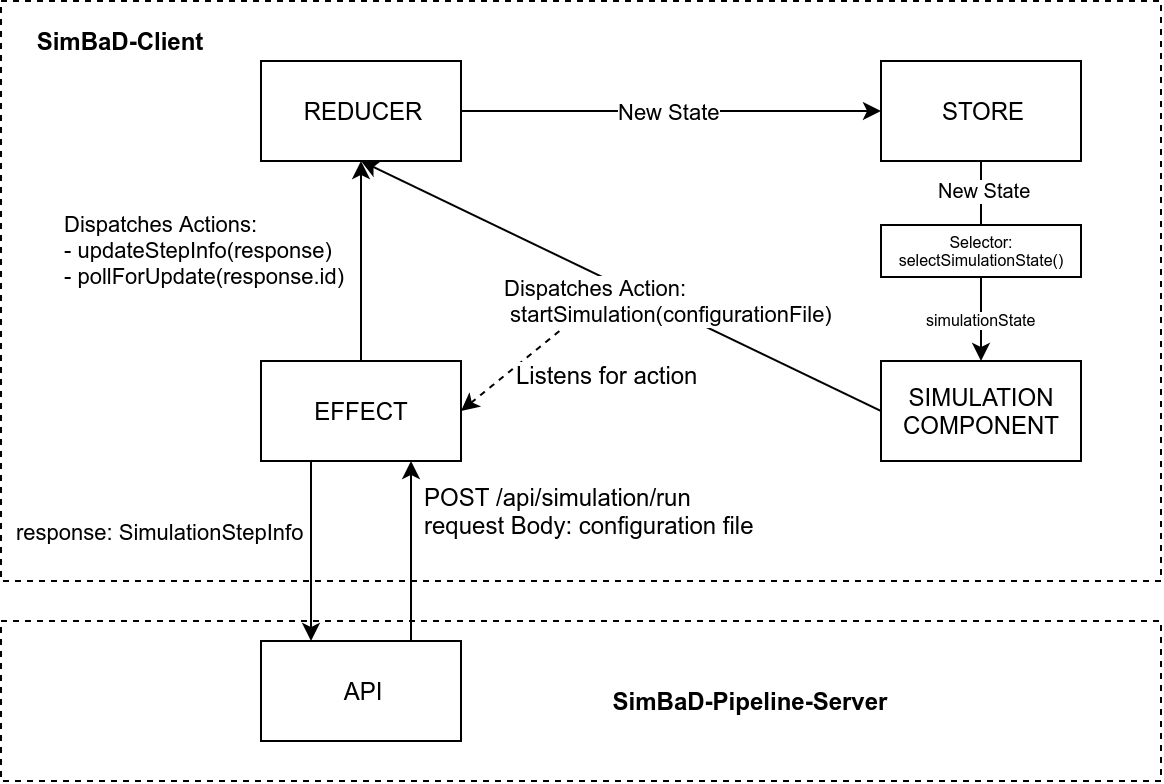
\includegraphics[width=0.9\linewidth]{diagrams/ngrx.png}
	\caption{Example of NgRX flow in SimBad-Client}
	\label{fig:ngrx}
\end{figure}
Reactive programming works very well with store architecture. The store can be thought of as a client-side database, where all data needed by application resides. The store reflects the complete state of application.
NgRX uses the RxJS library heavily - the store itself is an obervable, an components need to subscribe to the store observables to get the data. Store architecture solves problem of passing data between components.
In angular, data can be passed between components in server ways - from parent to child using Input() member variables, from child to parent using EventEmmiters() and between unrelated components using services. Problems arise when data needs to be passed several levels down in component tree - the root component has the data, and the leaf components needs this data, however for the component nodes along the way, that do not need the data, extraneous Input properties must be added. Store architecture bypasses that problem, by providing single source of truth or the store for all of the components to get data from and push data to. When actor such as user or server changes some data, this change is pushed to store, and automatically reflected in all of the components. NgRX is a library that provides tools to add store architecture to application. 
NgRx consists of several building blocks - actions, reducers, effects and selectors. The components can alter state of application or by dispatching actions to store. Actions consists of type - unique action identifier and payload - the data that is needed to change the state. Reducer is a pure function that accepts two arguments - current state of application and action. Reducer analyzes the action and returns new state that is a combination of previous state and action payload. Side effect can be something like making a http call, or showing a notification. The effects trigger when specific action is dispatched to store, and can be used to trigger side-effect based on those actions. Effects can also dispatch another action to the store, for example they can push response received from http call. Single effect can be triggered by multiple action, can dispatch multiple actions and single action can trigger multiple effects. The store can be pretty big object, and components need only a part of it. Selectors facilitate this by allowing the components to get or in other words "select" only parts of the store. In the figure \ref{fig:ngrx}, example NgRX flow trigerred by user starting the simulation is shown.

The user action, for example clicking a button, causes the component responsible for simulation view to dispatch startSimulation() action with simulation configuration file as its payload. This triggers two separate NgRX flows. In the first one, the action is passed to the reducer, and new state with added information that simulation has started is generated. Then the store observable emits new data and component receives a slice of this data, based on selector. The second flow starts with effect, that reacts to startSimulation Action being triggered. This effect makes then POST request to Simulation-Pipeline-Server to start simulation, and receives the information about the first simulation step - the SimBaD-CLI step. Effect then dispatches two actions with, response as a payload, one to update step info in store, and one to start polling for step info changes. Those actions then are handled by reducer, new store state is emitted and passed to component. If dispatched actions trigger any effects, another flow starts.
\subsection{Configuration editor view}
To start simulation process user needs to pass simulation configuration file or SCF. This file has tree-like structure and contains various objects and parameters that control the simulation process. Although those objects need have predefined value types, ranges, or enums, the exact definitions did not exists, and had to be created. Detailed description of this file and how to add new parameters to simulation can be found in appendix \ref{appendix:A}.
\begin{figure}[h!]
	\centering
		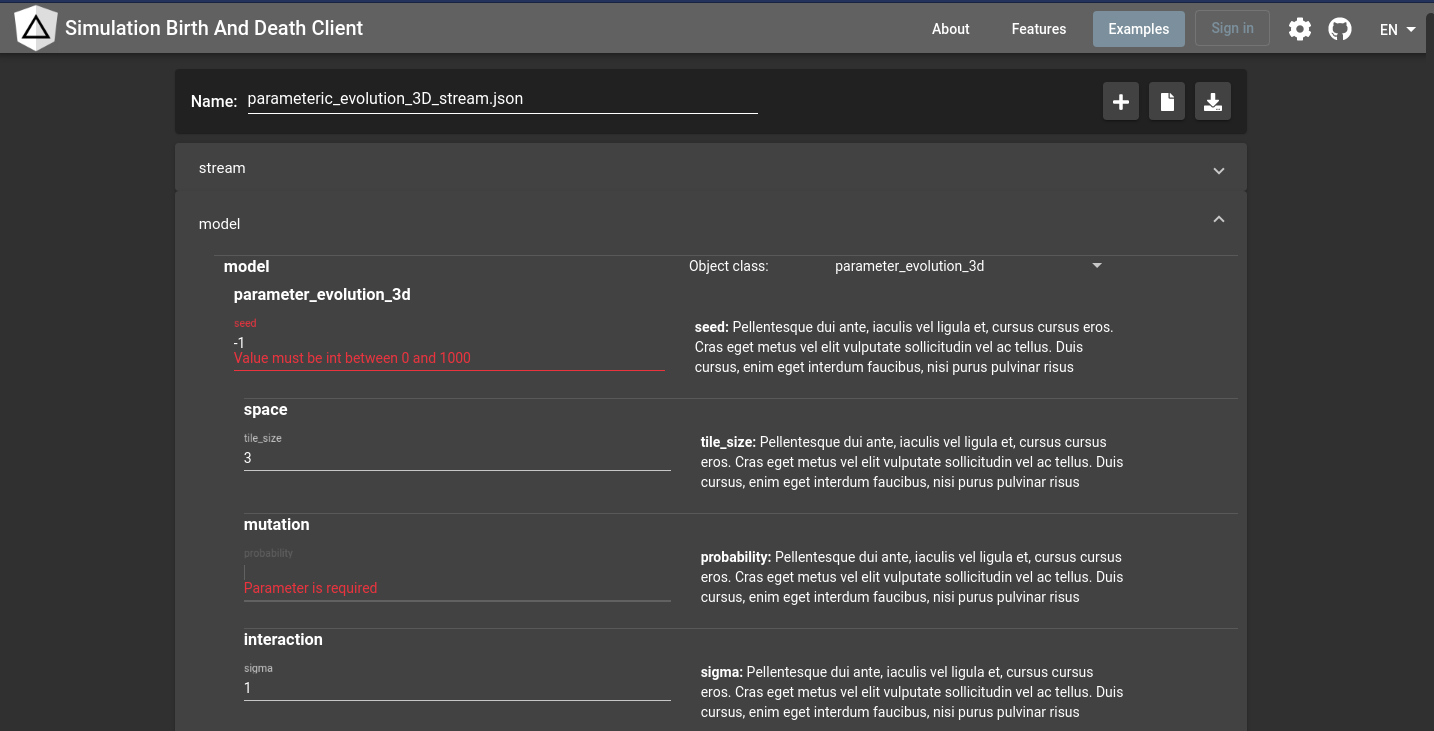
\includegraphics[width=0.9\linewidth]{screens/conf-view.png}
	\caption{The configuration editor view}
	\label{fig:conf-view}
\end{figure}
To enable user to generate valid configuration, configuration editor was created. Configuration editor generates forms that validate the parameter values entered by user against their definitions. The form has tree structure that maps to configuration. Additionally, each form input associated with parameter displays validation messages, and parameter description. The form is generated dynamically, and adding or changing definition in object definition does not break the form, though it requires to rebuild application. The user can create new configuration, and download and upload the configuration from .json file.  The SimBaD-CLI supports two file formats: .json and .simbad which is an alias to default boost:tree format. As the changes in configuration are dispatched to store, the configuration can be shared between different components. 
\begin{figure}[h!]
	\centering
		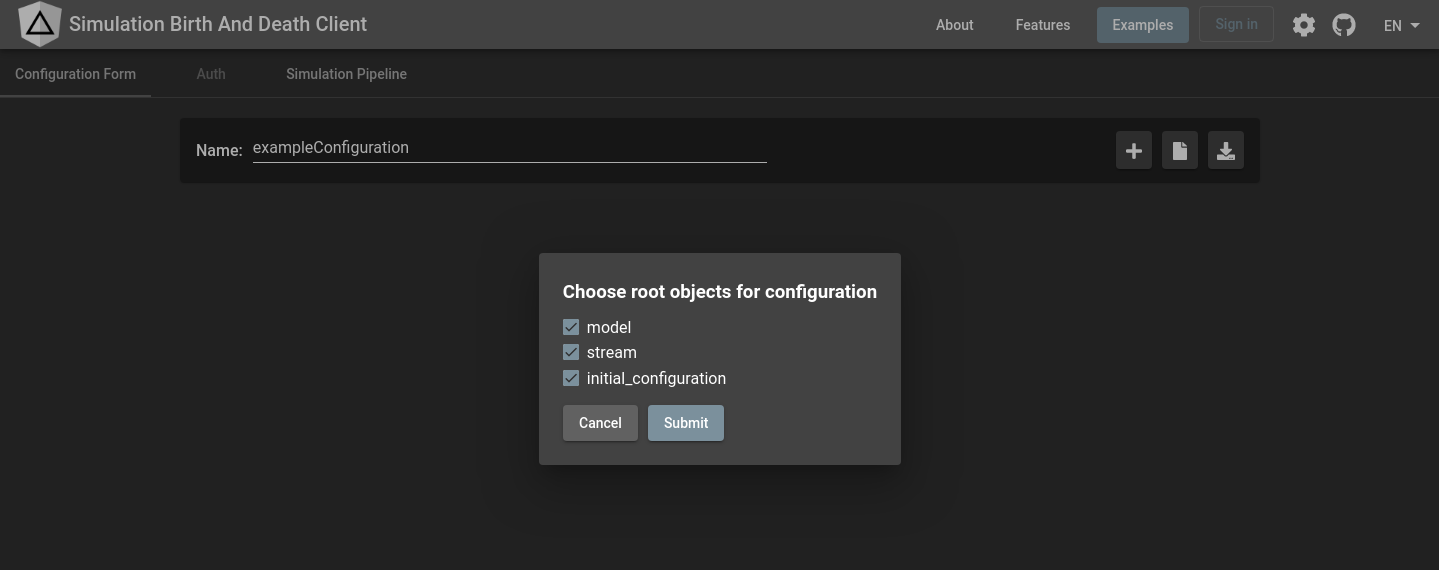
\includegraphics[width=0.9\linewidth]{screens/configuration-view-modal.png}
	\caption{Creating new configuration}
	\label{fig:conf-view-new}
\end{figure}
\subsection{Simulation pipeline view}
The second view of the application is the view that allows to monitor the simulation process. User can start simulation pipeline using this view. To start it, user can upload configuration file, or when present in store, use the previously edited configuration file. Additionally, user is able to load the results of last simulation. Each major change in step such as finishing or starting a step is accompanied by proper notification.
The simulation pipeline view consists of 3 main components, each responsible for different simulation step. Each of those components allows to view the current simulation status with information such as current step runtime status, the context of a step, and when step finishes, the resulting output files (also called simulation artifacts). Each artifact can be downloaded in .zip form, and for images, it can also be displayed. For the SimBaD-CLI view, visible in the figure \ref{fig:sp-cli}, additional metrics regarding the process executing the simulation are displayed - the CPU usage and ram usage. 
\begin{figure}[h!]
	\centering
		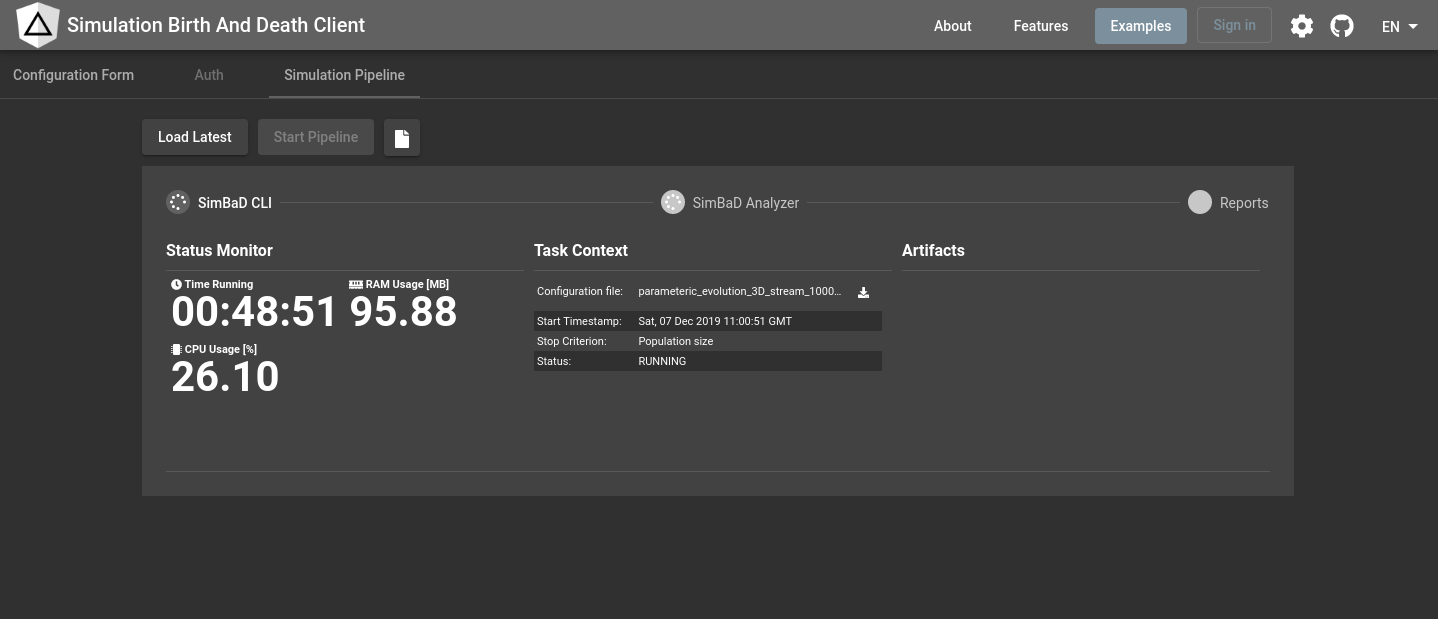
\includegraphics[width=0.9\linewidth]{screens/cli-view.png}
	\caption{Simulation pipeline view: CLI step}
	\label{fig:sp-cli}
\end{figure}
For the analyzer-view, there's a link to the Spark UI dashboard and progress bar that displays information about total progress of analyzer job, based on already created artifacts. This view can be seen on the figure \ref{fig:sp-analyzer}.
\begin{figure}[h!]
	\centering
		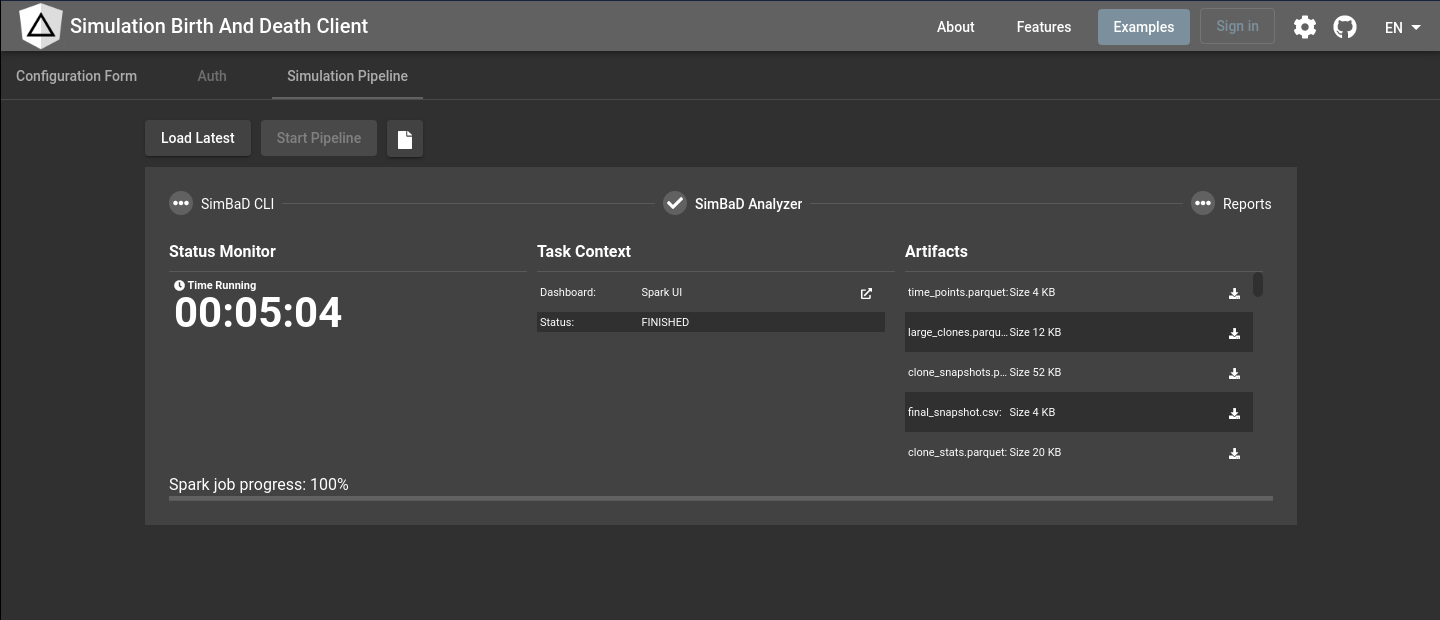
\includegraphics[width=0.9\linewidth]{screens/analyzer-view.png}
	\caption{Simulation pipeline view: Analyzer step}
	\label{fig:sp-analyzer}
\end{figure}
Finally the last step of this view is the report step. Apart from option to download the resulting plots, the user has also option to display the plots in browser. Example display of such plot is shown on the figure \ref{fig:sp-report-muller}.
\begin{figure}[h!]
	\centering
		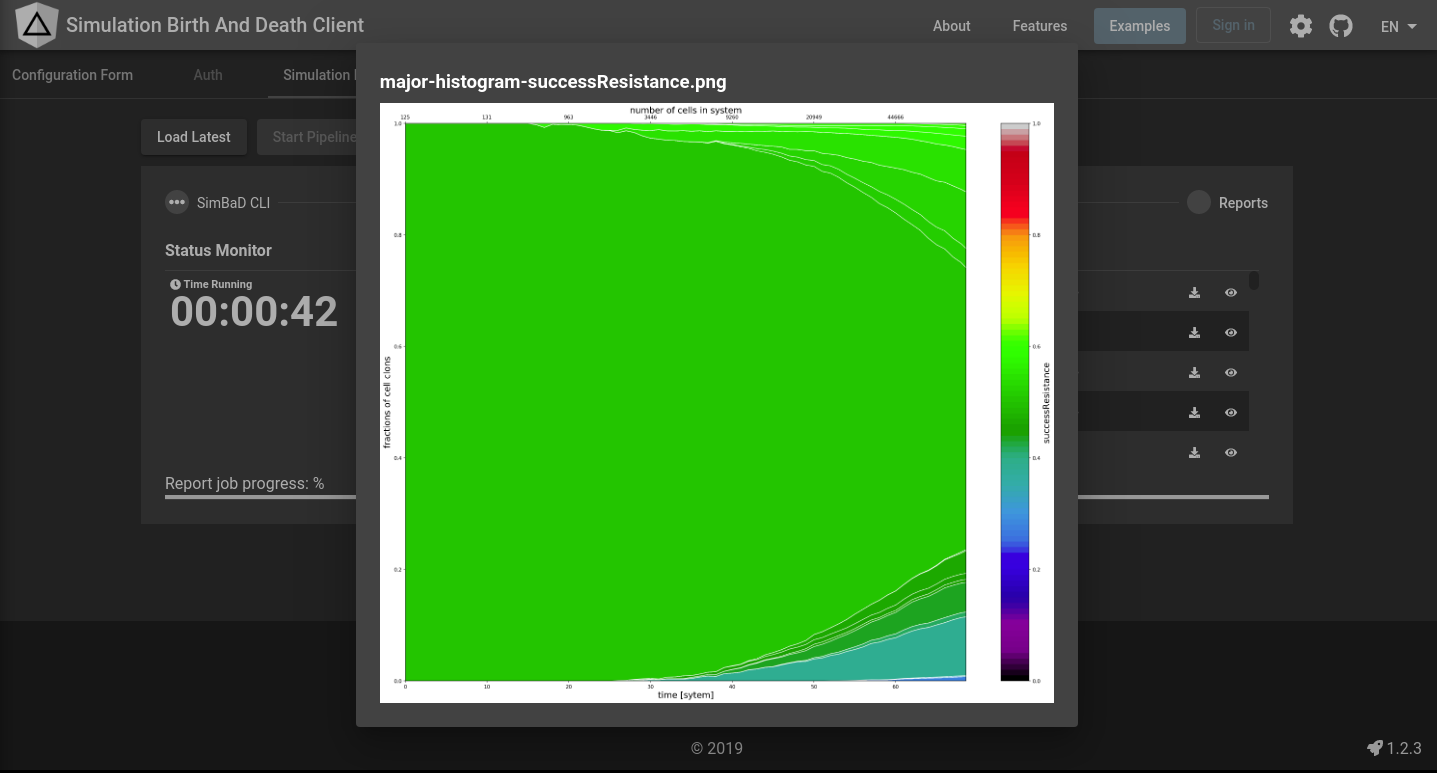
\includegraphics[width=0.9\linewidth]{screens/report-view-muller.png}
	\caption{Report view: mullerplot}
	\label{fig:sp-report-muller}
\end{figure}
\newpage
\subsection{Serving the client}
To server application from docker contaienr first it is necessary to build it. The application can be build in two ways- the development build and the production build. The development build contains non minified code with sourcemaps that is suitable for debugging.  Minification is a process of removing redundant data from the code (such as whitespace, comments or verbose function and variable names). and sourcemaps are files that map compressed and transpiled javascript code to its original source files. Such build should not be server to the user, as it not optimized in size, and contains informations valuable only to developer. The production on the other hand, reduces the size of the bundle applying minification tree shaking and ohter techinques. Such build is suitable to be actuall served to user but needs an actual server to host it. There are many http servers, but for the purpose of this application the nginx was used. Apart from serving the files, the nginx also is used as reverse proxy to SimbAd-Pipeline-Server. 
There are two steps to create docker image for this component. First, all of the npm packages necesary to build the application must be installed, and after building it, the resulting files must be copied to the /usr/share/nginx folder. To avoid increasing the image size the docker multi-stage builds feature was used. The dockerfiles for this component is visible on listing.
\begin{lstlisting}[label=list:sc-docker,caption=Dockerfile used to build SimBaD-Client, basicstyle=\footnotesize\ttfamily]
FROM node:11.1.0 as npm_builder
COPY ./package.json /usr/simbad-client/app/package.json
COPY ./package-lock.json /usr/src/app/package-lock.json

WORKDIR /usr/simbad-client/app
RUN npm install --silent

FROM npm_builder as builder
COPY . /app
ENV PATH /app/node_modules/.bin:$PATH
WORKDIR /app
RUN npm run build

FROM nginx
COPY --from=builder /app/dist/projects/simbad-client /usr/share/nginx/html
\end{lstlisting}
Dockerfile is split into three stages, the first npm\_builder extends the community image with installed NPM and node.
The package.json files containing client dependencies are copied onto the file and the packages from this file are installed. The second stage is builder, used to generate production build. The last stage is Nginx. It starts with nginx image from Dockerhub, to which the resulting build files are copied. The size of resulting image is the size of Nginx image + the size of build output - it does not have all of the node toolchains or node modules installed, and that saves over 1GB of disk space.
\section{SimBaD-Pipeline-Server}
This component is at the center of the simulation. It receives commands from the client and manages whole simulation process.
As discussed in chapter \ref{chapter:arch}, the SimBaD-Pipeline-Server must communicate with client using HTTP RPC API, store data in shared volume and sqlite database, and be able to communicate with existing components placed in same container, by executing the scripts and binaries directly, or with component in separate container, using HTTP RPC API and SSH. In the following sections the technology choices and inner mechanisms of working wil be discussed.
\subsection{Technology}
\subsubsection{Choice of framework}
Almost any programming language has some framework dealing with writing http servers. In that regard, the choice of the framework mainly depends on developer preference, as the http capabilities of the component can be created using any of those frameworks. The important factor is how well will the language work with existing binaries and scripts. As the server needs to be able to call python scripts and C++ binaries the choice narrows down to python web frameworks. Two most popular ones are Flask and Django. Out of those two, flask was chosen, mostly due to the fact that it gives developer much more freedom than Django, and allows to tailor application to specific use case, without imposing standard model, as Django. Django comes with extensive toolkit for serving HTML and server-side rendering, which is not needed for the SimBaD-Pipeline-Server, because it is used as web service, the actual serving of SimBad-Client is delegated to Nginx.
The flask is extendable but that also means that it needs to be manually extend to fit the needs, and the features like splitting the api routes into separate files or setting up ORM need to be done manually.
\subsubsection{ORM}
To save information about simulation ORM was used with help of SQLAlchemy. Overall simulation information was divided into several objects. Each simulation step generates output files, such files are represented by the Artifact object. This object has information about the path to actual file in the shared filesystem, which simulation and which simulation and which step generated the artifact, its size and timestamp when it was created. Individual simulation steps are represented by SimulationStep object. This object has information about current state and runtime info, resulting artifacts, and timestamps associated with step. Definition of SQLAlchemy model can be seen on listing.
\begin{lstlisting}[label=list:sp-sqlalchemy,caption=SimulationStep SQLAlchemy model, basicstyle=\footnotesize\ttfamily]
class SimulationStep(Base):
    __tablename__ = 'steps'
    RELATIONSHIPS_TO_DICT = True

    id = Column(Integer, primary_key=True)
    simulation_id = Column(Integer, ForeignKey('simulations.id'))
    started_utc = Column(DateTime)
    finished_utc = Column(DateTime)
    origin = Column(String())
    celery_id = Column(String())
  
    cli_runtime_info = relationship(
        "CliRuntimeInfo", 
        uselist=False, 
        backref="steps"
    )
  
    analyzer_runtime_info = relationship(
        "AnalyzerRuntimeInfo", 
        uselist=False,
        backref="steps"
    )
  
    artifacts = relationship("Artifact", backref="steps")
    
    def __json__(self):
        return ['id', 'simulation_id', 'started_utc', 'finished_utc',
                'origin', 'artifacts', 'cli_runtime_info',
                'analyzer_runtime_info']
\end{lstlisting}
SimualtionStep model extends the Base SQLAlchemy class which enables access to SQLAlchemy functionality, such declaring tables, primary keys or relationships between object. The \_\_json\_\_ method is used, when model is serialized to json, for example, for status responses to client. The list it returns defines which properties will be in serialized object. 
\subsubsection{Task queue}
Waiting for simulation to finish, before returning some sort of response to the client is not feasible, as the simulation process takes a lot of time, the http request should not be open for that long, and the user is deprived of simulation progress updates. To solve that, after receiving the server should start running the simulation in background, and return confirmation that simulation is started, along with other information that enables the client to poll for status changes.
Though only one simulation process should be run at a given time, multiple simulations should be able to be scheduled by multiple clients for later execution, and that calls for simulation task queue. To enable that functionality, Celery framework was used. Celery allows to schedule and execute tasks in synchronous and asynchronous way. At the start of the server, it searches for tasks in code(annotated by @celery.task), and starts worker threads that will execute those tasks.
To queue task, celery needs a way to transport messages, also called a messagge broker. The two main choices for brokers are RabbitMq and Redis. As Celery has support for each of those brokers, the primary factor was the size of docker image, and as the size of official Redis image is slightly smaller, Redis was chosen.
Celery allows to compose primitive celery tasks into different ways, to change the order of execution. Tasks in celery chains are executed in sequence, and the output of previous task is passed as first argument of current task, which is a perfect solution of simulation pipeline. Example of such chain is shown on listing \ref{list:sp-celery-chain}. 
\begin{lstlisting}[label=list:sp-celery-chain,caption=Celery chain - Main Simulation task, basicstyle=\footnotesize\ttfamily]
@celery.task(name='SIMBAD-SIMULATION-MAIN')
def run_simulation(artifact_id) -> AsyncResult:
    result = chain(
        cli_step.s(artifact_id),
        analyzer_step.s(),
        reports_step.s()
    ).apply_async()
    return result
\end{lstlisting}
The celery group allows to execute task in parallel, which is useful in the report step, as each report script can be executed independently. Celery groups, however cannot be chained together, so for plots the main primitive that was uses was chord. Chord is a task that is executed after all of the task in groups are executed. Example of chord is shown on the listing \ref{list:sp-celery-chord}. The chordfinisher task on the listing is a dummy tasks, and its used as a workaround for inability to chain groups.
\begin{lstlisting}[label=list:sp-celery-chord,caption=Start simulation endpoint, basicstyle=\footnotesize\ttfamily]
@celery.task(bind=True, name='SIMBAD-MAJOR-CLONES-MULLERPLOT-STATS')
def major_clones_mullerplot(self, workdir: str):
    param_names = [
        'birthEfficiency',
        'birthResistance',
        'lifespanEfficiency',
        'lifespanResistance',
        'successEfficiency',
        'successResistance',
    ]

    tasks = []
    for name in param_names:
        tasks.append(major_clones_mullerplot_histogram.s(workdir, name))
    chord(tasks, chordfinisher.si()).apply_async()
    return workdir
\end{lstlisting}
Example of combining Flask endpoitns, ORM and Celery task together is shown on listing \ref{list:sp-api-run}. The endpoint shown, is the endpoint that starts the simulation process.
First, the configuration file is extracted from request body, and setup for new simulation process is started. The result of setup is Artifact representing the simulation configuration file. Id of object representing SimBaD-CLI step is extracted from artifact and passed to simulation task. The simulation task is started and background, changes to database are commited, CLI step object is serialized to json and returned as response to SimBaD-Client.
\begin{lstlisting}[label=list:sp-api-run,caption=Start simulation endpoint, basicstyle=\footnotesize\ttfamily, language=python]
@simulation_api.route('/start', methods=['POST'])
def start():
    request_data: dict = request_to_json(request)
    conf: Artifact = setup_workdir(request_data)
    db_session.begin()
    db_session.flush()
    step = db_session.query(SimulationStep).get(conf.step_id)
    task = run_simulation.delay(conf.id)
    step.celery_id = task.id
    db_session.commit()
    return jsonify(step)
\end{lstlisting}
\subsection{Task executors}
For different configurations, different components of simulation pipeline can be placed on different docker containers or even on different machines. To enable easy switch between ways of executing certain task, the task executor interface was proposed. 
\begin{lstlisting}[label=list:sp-ex-base,caption=Base executor, basicstyle=\footnotesize\ttfamily, language=python]
class BaseExecutor:
    def __init__(self):
        self.is_finished = False
        self.result = None
        self.status = None

    def execute(self, in_file: Artifact) -> None:
        pass

    def cleanup(self) -> None:
        pass
\end{lstlisting}
This interface has to be implemented for each object managing simulation step. The main three implementations of this interface are LocalExecutor, HttpExecutor and SSH Executor. Use of task executors in celery tasks split the responsibilities - celery task acts as a client that starts task and periodically asks for updates or results, and the task executor act as a server, that actually executes the task. Because the celery task does not actually executes the task but rather uses an interface, the way which task are executed can be easily change. The interface is consistent for executors that run binaries and scripts locally and executors that make http calls to another server to start a task.
For the purpose of demonstrating such concept, each of those executors was implemented for a simulation step - LocalExecutor for SimBaD-CLI, HttpExecutor and SshExecutor for SimBaD-Analyzer step. The fragment of local executor implementation is shown on the listing \ref{list:sp-exec-local} and how executor is used from celery is shown on listing \ref{list:sp-exec-local-use}.
\begin{lstlisting}[label=list:sp-exec-local,caption=Fragment of LocalExecutor for SimBaD-CLI, basicstyle=\footnotesize\ttfamily, language=python]
def execute(self, in_file: Artifact) -> None:
    thread = threading.Thread(target=self.run_cli, args=[in_file])
    thread.daemon = True
    thread.start()
    return
    
def run_cli(self, conf: Artifact) -> None:
    self.status.step_id = conf.step_id
    out_path = '{}/cli_out.csv'.format(conf.get_workdir())
    conf_path = conf.path

    with open(out_path, 'w') as f:
        process = subprocess.Popen(
            (self.executable_path, conf_path), 
            stdout=subprocess.PIPE
        )
        process_info = psutil.Process(process.pid)
        counter = 0
        for c in iter(lambda: process.stdout.read(1), b''):
            counter += 1

            if counter % 1000000 == 0:
                memory = process_info.memory_info().rss / 1000000
                cpu = process_info.cpu_percent()
                self.status.memory = memory
                self.status.cpu = cpu
                # TODO: parse some additional status data from stderr?

            line = c.decode('utf-8')
            f.write(line)
\end{lstlisting}
As long as the specific executor is implemented for task, it can be used. Which executor is used to which task, as well as other configuration options can be set using docker .env files, wich will be described more in section \ref{sec:dockerconf}.
\begin{lstlisting}[label=list:sp-exec-local-use,caption=Use of LocalExecutor for SimBaD-CLI step, basicstyle=\footnotesize\ttfamily, language=python]
@celery.task(bind=True, name='SIMBAD-CLI')
def cli_step(self, artifact_id: int) -> int:
    conf: Artifact = db_session.query(Artifact).get(artifact_id)
    ...
    executor: BaseExecutor = get_cli_executor()
    executor.execute(conf)

    while executor.is_finished is not True:
        db_session.begin()
        runtime_info.cpu = executor.status.cpu
        runtime_info.memory = executor.status.memory
        db_session.commit()
        sleep(POLLING_PERIOD)

    result: Artifact = executor.result
    ...
    return result.id
\end{lstlisting}
The SSH Executor is functionally identicall to HTTP Executor, the only difference that before the first connection, it opens SSH tunnel to remote server, using the SSHTunnelForwarder from sshtunnel python library. 
\section{SimBaD-Analyzer-Server}
Extracting component to separate docker container requires adding http layer on top of it, which will be used by the aforementioned Http and SSH TaskExecutors on the pipeline server. In the proposed system, this such layer, named SimBaD-Analyer-Server was added on top of the SimBaD-Analyzer component. 
\subsection{Technology}
To maintain consistency across apps, and other reasons stated in frameworks overview in section, Flask was selected as a framework of choice for managing http api. The API definitions, as it was the case server-client communication, were defined using OpenAPI. Python and Flask dependencies were added tp existing docker image containing spark ecosystem and built Simbad-Analyzer jars. Propsed architecture assumes that all of the components have access to the same shared volume, to make that possible for containers on separete hosts, sshfs docker extension was added. This extensions allows to create shared docker volume, and allow acces to it through ssh connection.
\subsection{Integration with Spark}
In its structure, the extension to analyzer is very similar to TaskExecutor. Properties and methods of task executor are now mapped to endpoints - the execute method is now the /api/analyzer/start endpoint, the result property is now a /api/analyzer/result endpoint and so on. Making a POST request to /api/analyzer/start endpoint, with path to the output file of SimBaD-CLI, starts the step. Before submitting the job to spark, checkpoints and spark warehouse that might have been created by previous simulation run need to be cleared.
\begin{lstlisting}[label=list:sp-exec-local-use,caption=Use of LocalExecutor for SimBaD-CLI step, basicstyle=\footnotesize\ttfamily, language=python, numbers=left]
@app.route('/api/analyzer/start', methods=['POST'])
def start():
    global analyzer_status
    if analyzer_status['status'] is 'BUSY':
        return {"status": "failed"}, 402
        
    request_data: dict = request_to_json(request)
    path: str = request_data['path']
    analyzer_status['status'] = 'BUSY'
    start_analyzer(path)
    return "OK", 202
\end{lstlisting}
Submitting tasks to spark is done through running shell commands. Two commands must be run, first to read the generated by the CLI and second to analyze it. Method executing this command can be seen on listing. After submitting the Analyzer job to spark, daemon starts in background that periodically updates the progress of simulation, by checking how many of the required files files were created. If all of the required files were created, the global result variable is set to list of paths of created files, and can be retrived by TaskExecutor running on SPS through /api/analyzer/result endpoint.
\begin{lstlisting}[label=list:sp-exec-local-use,caption=Use of LocalExecutor for SimBaD-CLI step, basicstyle=\footnotesize\ttfamily, language=python, numbers=left]
def start_analyzer(path: str) -> None:
    ...
     reader_cmd = "spark-submit" \
                  " --master local " \
                  "--class analyzer.StreamReader " \
                  "/jar/analyzer.jar {} {}"\
                  .format(path, stream_dir)
    reader_process = subprocess.Popen(reader_cmd, shell=True)
    reader_process.wait()
    analyzer_cmd = "spark-submit" \
                   " --master local " \
                   "--class analyzer.Analyzer /jar/analyzer.jar {} {}"\
                   .format(stream_dir, spark_out_dir)
    subprocess.Popen(analyzer_cmd, shell=True)
    thread = threading.Thread(target=update_runtime_info)
    thread.daemon = True
    thread.start()
    return
\end{lstlisting}
\section{Docker containers for components}
The first container that needs to be added is the contaienr with nginx that hosts the SimBaD-Client code. The Simbad-Pipeline-Server component requires three docker containers to run. First container serves the http api that is used by the client. Second container runs the Celery worker, that executes scheduled task. Those two containers share the same image. The third component is a Redis image, that acts as a message broker for Celery. The last container is a container for simbad-analyzer-server, containing the HTTP API extension and SimBaD-Analyzer. The diagram visualizing all of the containers can bee seen on the figure \ref{fig:docker-containers}.
\begin{figure}[h!]
	\centering
		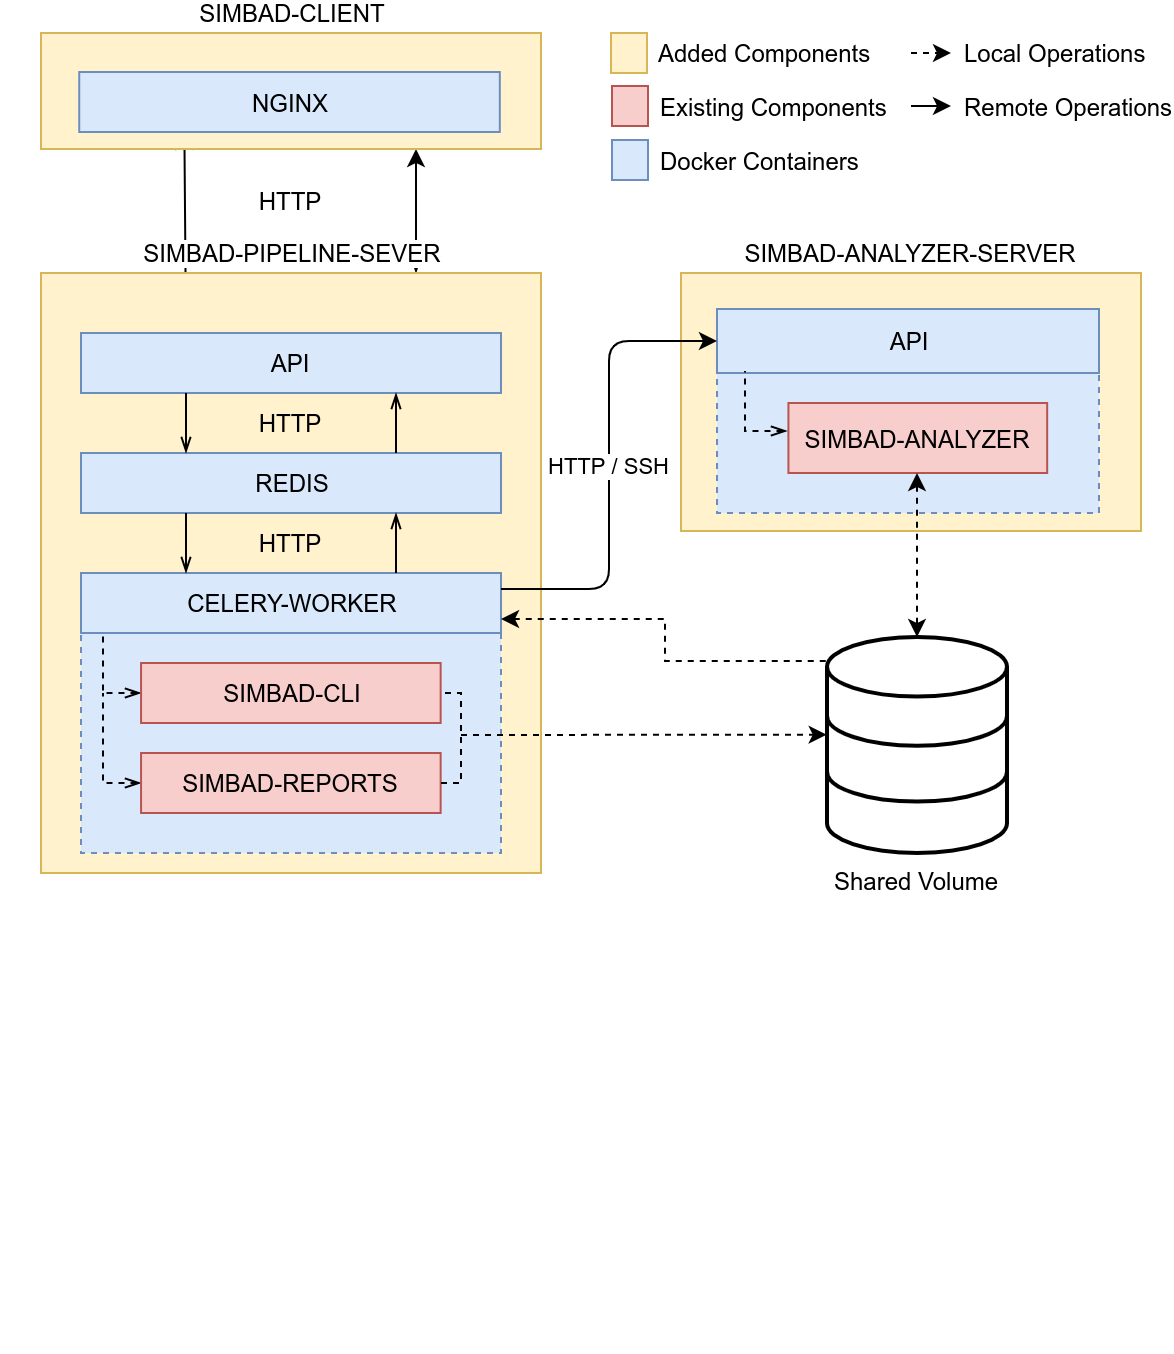
\includegraphics[width=0.9\linewidth]{diagrams/docker.png}
	\caption{Diagram of docker-compose containers}
	\label{fig:docker-containers}
\end{figure}
When simulation systems grows in a decoupled way, the number of docker container to manage also grows. To aid managing these containers, docker-compose was used. This tool can be used to define and manage application consisting of several components, placed on separate docker containers. The definition of application is placed in single docker-compose.yaml file. One can define services, shared volumes and networks in this file, and the start whole application using single commands. Contaienrs are build from images that can be defined using Dockerfiles or downloaded from DockerHub. Additionally, the network and volume definitions also can be placed in this file. Developing such system causes a need for two separate docker-compose files, one for the developer, that builds docker images from source, and one for user, so called, that pulls prebuild images from DockerHub. The docker-compose file that defines all of the simulation components using prebuild images is depicted on listing.  \ref{list:docker-compose}. 
\begin{lstlisting}[label=list:docker-compose,caption=prod-docker-compose.yaml file, basicstyle=\footnotesize\ttfamily, numbers=left, escapechar=|]
version: '3.4'
services:
  client:
    image: jsokolowski/simbad-client
    container_name: simbad-client
    ports:
      - "8080:80"
    volumes:
      - ./nginx.conf:/etc/nginx/nginx.conf
  pipeline:
    image: jsokolowski/simbad-pipeline-server |\label{line:sp}|
    container_name: simbad-pipeline-server
    command: python entrypoint_api.py --port 8081 --debug
    env_file:
      - ./docker.env
    ports:
      - "8081:8081"
    volumes:
      - ../data:/usr/data
  worker:
    image: jsokolowski/simbad-pipeline-worker
    container_name: celery-worker
    links:
      - analyzer-server
    command: celery worker -A entrypoint_celery.celery --loglevel=info
    env_file:
      - ./docker.env
    volumes:
      - ../data:/usr/data
  analyzer-server:
    image: jsokolowski/simbad-analyzer-server
    container_name: simbad-analyzer-server
    command: python3 app.py --port 5000 --debug
    env_file:
      - ./docker.env
    volumes:
      - ../data:/usr/data
      - ./log4j.properties:/opt/spark-2.4.3-bin-hadoop2.7/conf/log4j.properties
    ports:
      - "5000:5000"
      - "4040:4040"
  redis:
    image: redis:alpine
    container_name: redis
    ports:
      - "6379:6379"
\end{lstlisting}
All of the simulation component containers are defined under the "services" tag, for example, analyzer-server tag defines configuration of SimBaD-Analyzer-Server component. The image key, under the analyzer-server, specifies from where to pull the prebuild image. The "command" key specifies what command needs to be executed after container is started. The env\_file key specified the path to file with environmental variables, that need to be set inside of container OS. This file is also primary method of configurating the system and will be described in more detail in section  \ref{sec:configuration}. Shared volumes and files that need to be placed inside container can be defined using the volmes key. First entry under that key is a shared volume, where the simulation files will reside. The " ../data:/usr/data" syntax, means that the local data folder will be mounted as /usr/data folder inside of the container. The "value:value" syntax in general can be interpreted as "HOST:CONTAINER". Similiary, second entry under this key copies local configuration file for log4j, that is used to configure logging in spark. The last key is ports which is used to define which ports need to be exposed in container. The syntax "5000:5000" means that the through port 5000 on docker host, it is possible to access port 5000 on docker container. Port 5000 on this container exposes the  Simbad-Analyzer-Server API and port 4000 is used to access SparkUI dashboard.
Using the development version of the docker-compse.yaml file developer can easily make changes to system component, build the images from source, and publish them on DockerHub.
\section{System Configuration}
Two main sources of configuration are the docker-compose files and .env files. Form the compose files it is possible to specify ports and paths to data. The .env file contains the definition of environment variables that will be set in , that every container is passed to. In those files, there are more adavanced settings, mostly for power users, such as which executor will run which task, the updates polling period, or external drives to be mounted via sshfs.
\subsection{Remote host}
To enable running components on separate machines, docker configuration most be modified. Example steup for such configuration could be Simbad-Analyzer-Server running on one linux machine, and all other components running on the other.
For the sake of example, those two machiens will be on the same network, the SAS at 192.168.0.32 and the rest at 192.168.0.31. First step to enable that, is to extract the SAS container to a separate docker compose file, visible on the listing \ref{list:docker-split}. The entry under the analyzer-server key in original docker-compose file should be removed, to prevent running redundant containers.
\begin{lstlisting}[label=list:docker-split,caption=prod-docker-compose.yaml file, basicstyle=\footnotesize\ttfamily, numbers=left, escapechar=|]
version: '3.4'
services:
  analyzer-server:
    image: jsokolowski/simbad-analyzer-server
    container_name: simbad-analyzer-server
    command: python3 app.py --port 5000 --debug
    env_file:
      - ./docker.env
    volumes:
      - sshfs:/usr/data
      - ./log4j.properties:/opt/spark-2.4.3-bin-hadoop2.7/conf/log4j.properties
    ports:
      - "5000:5000"
      - "4040:4040"
    network_mode:
      host
volumes:
    sshfs:
      name: sshfs
      driver: vieux/sshfs:latest
      driver_opts:
        sshcmd: "user@192.168.0.31:/home/user/simbad/data"
        password: "password"
\end{lstlisting}
The network mode is set to host, to make the container available from outside. It's worth noting, that this option works only on docker for linux. Additionally to make the filesystem available to both machines, the SAS must mount the filesystem of other machine, at the same mountpoint. This is done through docker sshfs docker extension. First, in the root volume key, the ssfs drive is defined, and then, it is mounted in the volume key under analuzer\_server. Second file that needs to be edited is the docker environment file. In this file the address and port to SAS must be entered, and the analyzer TaskExecutor must be set to HTTP. Fragment of such env file can be seen on the listing \ref{list:docker-split-env}
\begin{lstlisting}[label=list:docker-split-env,caption=prod-docker-compose.yaml file, basicstyle=\footnotesize\ttfamily, numbers=left, escapechar=|]
...
SIMBAD_ANALYZER_HOST="192.168.0.32"
SIMBAD_ANALYZER_PORT="5000"
SIMBAD_ANALYZER_EXECUTOR=HTTP
...
\end{lstlisting}
To start the system, user would need to enter docker-compose up on both machines.
\label{sec:configuration}
\chapter{Results}
\label{chapter:5}
Proposed system was installed successfully on \textit{Windows} and on \textit{GNU\textbackslash Linux}. Installation process is simplified and after downloading the source code user can install the system with single command. The complete installation instructions for \textit{Windows} and \textit{GNU\textbackslash Linux} can be found in appendix \ref{appendix:B}. The user can easily start, and monitor the simulation process, without any significant technical knowledge.
The results simulation run are over 20 plot images, visualising the changes of simulation state in time. Fragment of example results can be visible on figures \ref{fig:result-size}, \ref{fig:result-entropy} and \ref{fig:result-lifespan}.
\begin{figure}[h!]
	\centering
		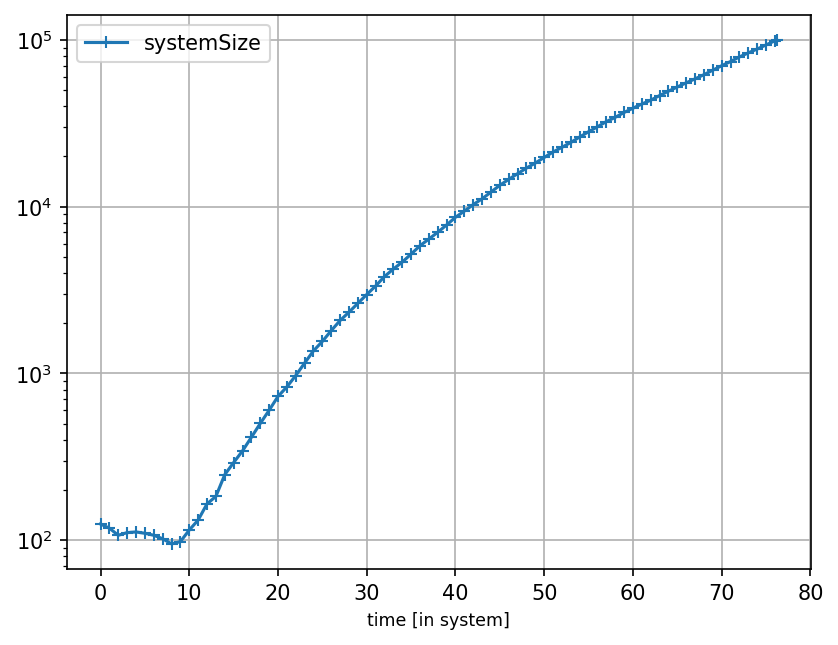
\includegraphics[width=0.7\linewidth]{reports/systemSize.png}
	\caption{Example result report: systemSize plot}
	\label{fig:result-size}
\end{figure}
\begin{figure}[h!]
	\centering
		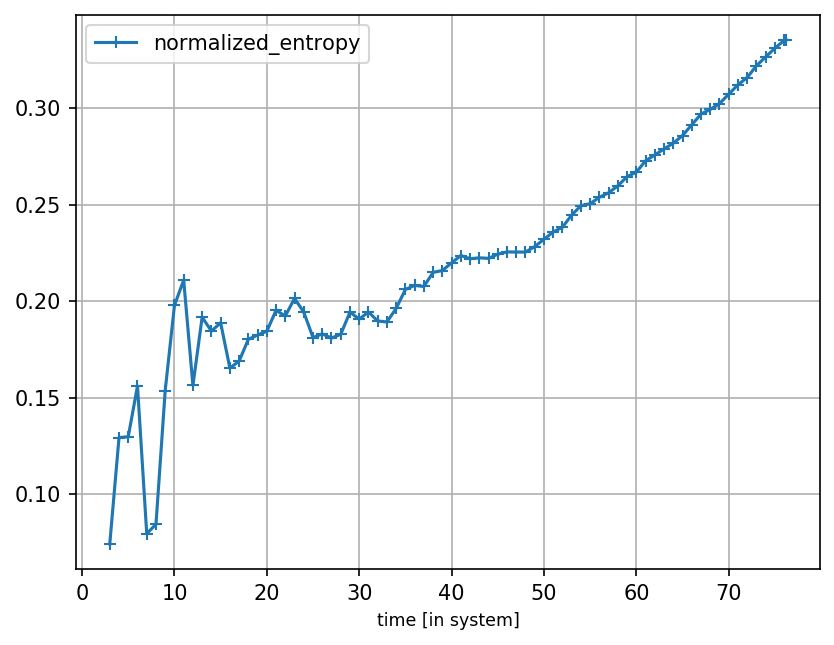
\includegraphics[width=0.7\linewidth]{reports/entropy.png}
	\caption{Example result report: entropy plot}
	\label{fig:result-entropy}
\end{figure}
\begin{figure}[h!]
	\centering
		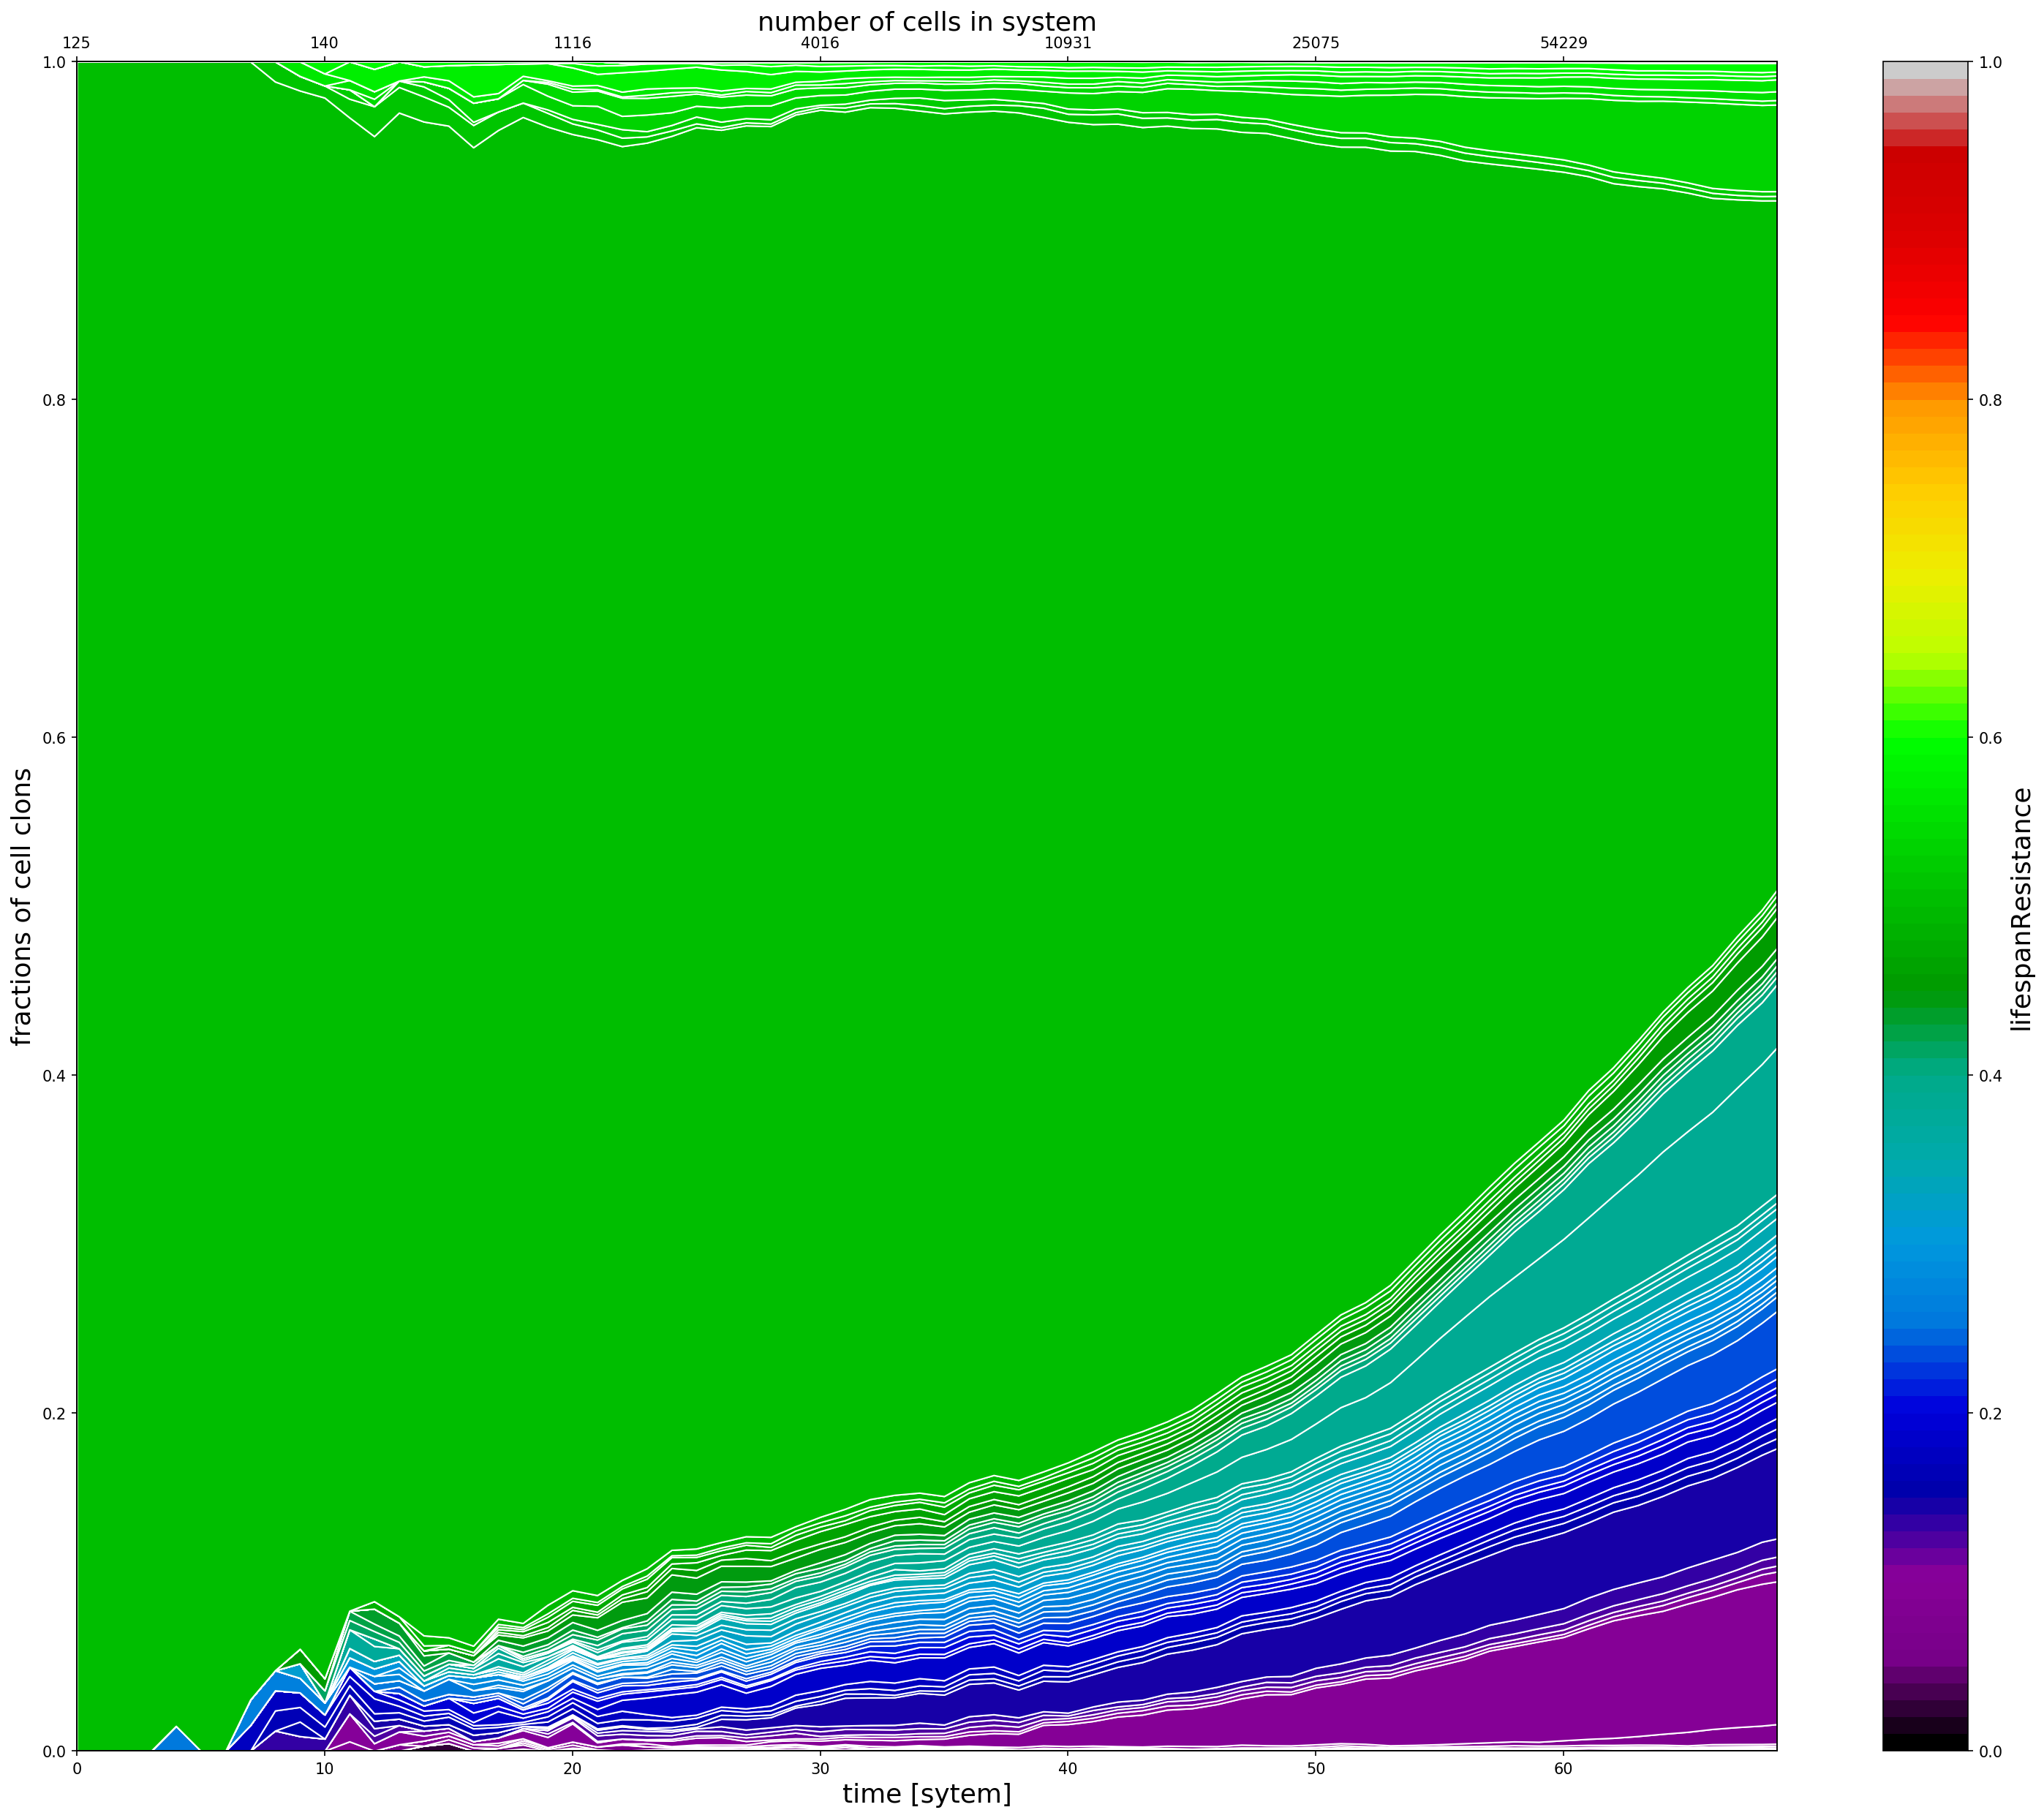
\includegraphics[width=0.7\linewidth]{reports/lifespanResistance.png}
	\caption{Example result report: lifespanResistance plot}
	\label{fig:result-lifespan}
\end{figure}

\newpage
\chapter{Conclusion}
\section{Encountered issues}
\subsection{Dead end of docker.host.internal}
\subsection{Growing size of containers}
\section{Future work}
\subsection{3D model of Cells}
From the simulation output, it is possible to generate 3D model of cancer cells in system. Currently, this model is rendered using CloudCompare. Final extension of the simulation pipeline would be to generate such model and render it in browser. The user could then rotate the cells, view its surface and cross-section. To manage such computationally-heavy processing, from client side a combination of WEB-GL and WASM could be used.
\subsection{WCSS integration}
Another important extension, is to integrate the proposed system with WCSS supercomputer. This would be possible through writing SSH Executors for each step, and from the SAS side, add switching between running the spark as subprocess, and submitting the job to internal WCSS queue.
\subsection{Better use of Celery}
Whole TaskExecutor concept can be made obsolete through better use of existing Celery Features. In Celery, multiple workers can connect to the same broker, and execute scheduled task. To achieve the same separation of concerns as in case of http extensions and task executors, multiple task queues can be defined. For example, separate task queue for CLI tasks and separate task queue for Analyzer tasks. Specific worker can be assigned to run only tasks from specific queue. In such configuration, celery manages the passing of the messages and results, instead of manually defining http extensions and endpoints.
\subsection{UI/UX}
There are many improvements and additions that can be made to the user interface. First one that comes to mind is a view that would allow to browse results of already completed simulations,as for now, only the latest result can be loaded. Another important addition would be a way to configure setup the system from the browser. The initial docker-compose up would start the client, and in client user, using some kind of configuration wizard would be able to setup the system. An array of small improvements can be made to existing UI components: possibility to search parameter in configuration editor, filter input for finding selected artifact, possibility to adjust the font size or fixing the flex-box in simulation view to fit on smaller screens and mobile devices. Another important addition, albeit requiring the modification of existing simulation components is displaying more accurate progress. The stop criterion for simulation can be number of cells in system, or elapsed time. The second option is trivial to implement, but the first one requires information about current cell number from SimBaD-CLI, and that currently is not given.
\subsection{CI}
Continous itnergration is very important for software development as it allows to make sure that system works in automated way. It also streamlines the release process, as each successfully master build could update hosted documentation and push new images to DockerHub. Currently some form of CI system is setup for two components, the SimBad-CLI and simbad-Client. Another step would be to add CI for other components, and add some form of integration tests for entire system. The tests would simulate user activity in the browser, but the simulation would be run on real components. 




%\bibliographystyle{plalpha}
\bibliographystyle{plabbrv}

\bibliography{bibliography}
\appendix
\chapter{Configuration objects definitions}
\label{appendix:A}
Parameters that can be defined in simulation configuration file are defined in \textit{configurationSchema.json} file. Simulation files have tree structure and consist of several root objects that have multiple child objects, but for simplicity and re-usability, in schema those parameters are defined as flat list.

\begin{lstlisting}[label=list:param-def,caption=Parameter definitions in schema, basicstyle=\footnotesize\ttfamily]
[
    "paramName1": {...},
    "paramName2": {...}
]
\end{lstlisting}

The order in which parameters are defined in schema does not matter, as long as all parameters that other parameters depend on are defined. There are several parameter types
\section{Simple parameter}
This parameter type consists of single floating, integer or string value. It cannot have any child parameters. Example of such parameters in simulation file - \textit{sigma}, \textit{gamma} and \textit{scale} are simple parameters.
\begin{lstlisting}[label=list:simple-param,caption=Simple parameter definition, basicstyle=\footnotesize\ttfamily]
"parameters": {
    "sigma": "5",
    "gamma": "2",
    "scale": "10"
}
\end{lstlisting}
Definition for such parameter in `configurationSchema.json` looks like this:
\begin{lstlisting}[label=list:simple-param-def,caption=Simple parameter definition, basicstyle=\footnotesize\ttfamily]
"sigma": {
    "type": "simple",
    "description": "Some parameter description",
    "parameterType": "int",
    "minValue": 0,
    "maxValue": 1000,
    "defaultValue": 1
},
\end{lstlisting}

\section{Enum parameter}
Enum parameter is parameter that changes its child parameters based on its class - \textit{saturation} is an example of such parameter - it has two possible classes \textit{`inverse\_generalized\_exponential} and \textit{genralized\_exponential}

\begin{lstlisting}[label=list:enum-param-ex1,caption=Enum parameter example, basicstyle=\footnotesize\ttfamily]
"saturation": {
    "class": "inverse_generalized_exponential",
    "parameters": {
        "sigma": "10",
        "gamma": "2",
        "scale": "1000"
    }
},
\end{lstlisting}

Same parameter with different class would look like this:
\begin{lstlisting}[label=list:enum-param-ex2,caption=Enum parameter example, basicstyle=\footnotesize\ttfamily]
"saturation": {
    "class": "generalized_exponential",
    "parameters": {
        "sigma": "5",
        "gamma": "2",
        "scale": "10"
    }
}
\end{lstlisting}
Definition for such parameter in schema:
\begin{lstlisting}[label=list:enum-param-def,caption=Enum parameter definition, basicstyle=\footnotesize\ttfamily]
"saturation": {
    "type": "enum",
    "description": "Some description",
    "possibleClasses": [
        "generalized_exponential",
        "inverse_generalized_exponential"
    ],
    "defaultValue": "generalized_exponential"
}
\end{lstlisting}
\section{Complex}
Complex - this parameter type has one or more simple, complex or enum children. In example below \textit{generalized\_exponential} is such parameter - it has 3 simple children.
\begin{lstlisting}[label=list:complex-param-ex,caption=Complex parameter example, basicstyle=\footnotesize\ttfamily]
"saturation": {
    "class": "generalized_exponential",
    "parameters": {
        "sigma": "5",
        "gamma": "2",
        "scale": "10"
    }
},
\end{lstlisting}
\textit{Mutator} is an example of complex parameter with complex children :
\begin{lstlisting}[label=list:complex-ex,caption=Complex parameter example, basicstyle=\footnotesize\ttfamily]
"mutator": {
    "efficiency": {
        "class": "uniform_step",
        "parameters": {
            "increase_length": "0.1",
            "decrease_length": "1.0"
        }
    },
    "resistance": {
        "class": "uniform_step",
        "parameters": {
            "increase_length": "0.1",
            "decrease_length": "1.0"
        }
    }
}
\end{lstlisting}
Definition of such parameter is analogous to enum parameter, but instead of \textit{possibleClasses} that parameter can have, array of \textit{childClasses} is defined:
\begin{lstlisting}[label=list:complex-def,caption=Complex parameter definition, basicstyle=\footnotesize\ttfamily]
"mutator": {
    "type": "complex",
    "description": "Mutator description",
    "childClasses": ["efficiency", "resistance"]
},
\end{lstlisting}
\chapter{Installation instruction}
\section{Windows}
\begin{enumerate}
    \item Install Docker for Windows using instructions from: \newline
    https://docs.docker.com/docker-for-windows/install/
    \item Enable hyper-v using instructions from: \newline
    https://docs.docker.com/docker-for-windows/install/
    \item Restart the computer
    \item Click Docker icon in tray and enable option "Switch to Linux Containers..." \newline
        \begin{minipage}{\linewidth}
            \centering
        	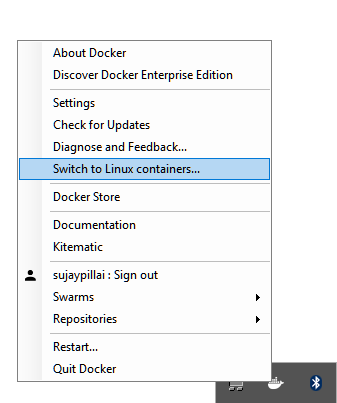
\includegraphics[width=0.4\linewidth]{instructions/systemtray.png}
        \end{minipage}
    \item Optional - open docker settings by clicking settings option and  in adavanced settings adjust how much resources can docker containers use
        \begin{minipage}{\linewidth}
            \centering
        	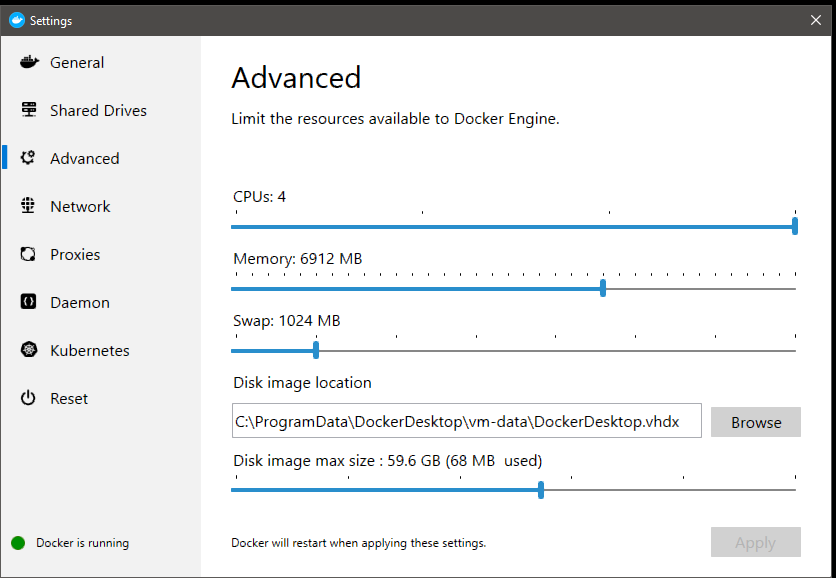
\includegraphics[width=0.4\linewidth]{instructions/res.PNG}
        \end{minipage}
    \item Clone or download repository from: \newline
     https://github.com/JakubSokolowski/simbad-monorepo
    \item Open powershell by pressing windows+R, typing "powershell" and pressing enter.
    \item From inside of powershell change directory to directory when the cloned repository is. The easiest way to do that is to find folder containing repository in Windows Explorer, type "cd " in powershell and drag and drop this folder onto powershell window. The command in powershell should now look like "cd C:\textbackslash Users \textbackslash Alice \textbackslash simbad\-monorepo". Press enter to execute it.
    \item While in cloned folder, enter command docker-compose -f docker/prod-docker-compose.yml up. This will start the download process - this operation may take around 15 mins depending on the internet connection and will download around 4GB of data. \newline
        \begin{minipage}{\linewidth}
            \centering
        	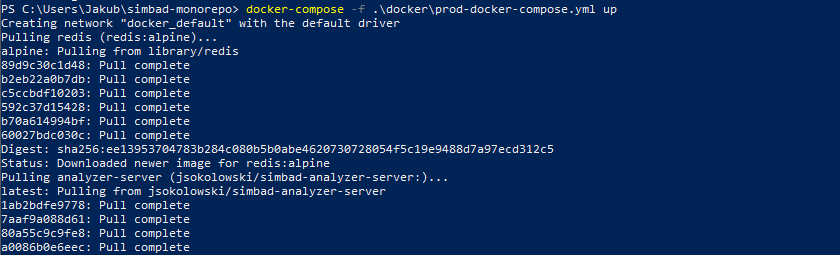
\includegraphics[width=0.9\linewidth]{instructions/docker2.PNG}
        \end{minipage}
    \item Docker will prompt you to enter password for, to grant access to host filesystem. Enter user password for each such prompt. \newline
    \begin{minipage}{\linewidth}
        \centering
        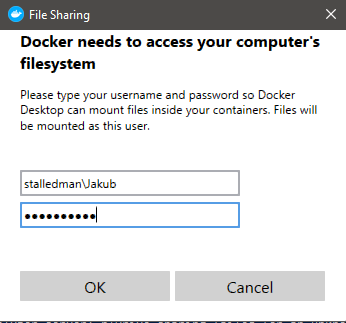
\includegraphics[width=0.5\linewidth]{instructions/docker3.PNG}
    \end{minipage}
    \item After command finishes executing, go to \textit{http://localhost:8080/\#/examples/simulation-pipeline } in browser.
    \item To stop, press ctrl+c in powershell
\end{enumerate}
\section{Linux}
\begin{enumerate}
    \item Install Docker using instructions from: \newline
    \textit{https://docs.docker.com/install/}
    \item Install Docker Compose using official instructions from: \newline
    \textit{https://docs.docker.com/compose/install/}
    \item Clone or download repository from: \newline
     https://github.com/JakubSokolowski/simbad-monorepo
    \item Open the terminal in the root folder of cloned repository
    \item Enter command docker-compose -f docker/prod-docker-compose.yml up. This will start the download process - this operation may take around 15 mins depending on the internet connection and will download around 4GB of data.
    \item Go to \textit{http://localhost:8080/\#/examples/simulation-pipeline } in browser
    \item To stop, press ctrl+c in terminal
\end{enumerate}

\chapterstyle{noNumbered}
\phantomsection % sets an anchor
\addcontentsline{toc}{chapter}{Indeks rzeczowy}
\printindex

\end{document}
